%\documentclass{book}\usepackage{sjtfonts}\usepackage{includegraphics}\usepackage{alltt}\usepackage{latexsym}
%\begin{document}\input{defs0}%		miradefs.tex 		    June 1994

% opening and closing a quoted Miranda section

\newcommand{\mira}{\noindent\hrulefill\nopagebreak\so}
\newcommand{\arim}{\nopagebreak\st\hrulefill\\}

% backslash in the Miranda environment
% Only feasible approach is to use \verb+\+
% in line!

%\newcommand{\bs}{$\mi\backslash\!\!$}
%\newcommand{\lbs}{\mbox{\verb+\+}}

% ignoring part of the input

\newcommand{\ignore}[1]{}

% a blank line in a Miranda section

\newcommand{\bl}{\mbox{\ }}

% Signalling a diffculty.

\definecolor{light-gray}{gray}{0.95}

\newcommand{\beware}[2]
 {\medskip\noindent\colorbox{light-gray}{\parbox{\textwidth}
 {\mbox{\large\textbf{#1}} \medskip\noindent\\ #2}\medskip\noindent}}

% Subscripting in Miranda text
\newcommand{\subscr}[2]{\mbox{${\mbox{\texttt{#1}}}_{\mbox{\texttt{#2}}}$}}

%\newcommand{\subscr}[2]{\mbox{${\mbox{\mi #1}}_{\mbox{\smtt #2}}$}}
\newcommand{\aone}{\subscr{a}{1}}
\newcommand{\atwo}{\subscr{a}{2}}
\newcommand{\ak}{\subscr{a}{k}}

\newcommand{\aoneone}{\subscr{a}{1,1}}

\newcommand{\eone}{\subscr{e}{1}}
\newcommand{\etwo}{\subscr{e}{2}}
\newcommand{\ei}{\subscr{e}{i}}
\newcommand{\er}{\subscr{e}{r}}

\newcommand{\fone}{\subscr{f}{1}}
\newcommand{\fl}{\subscr{f}{l}}

\newcommand{\gone}{\subscr{g}{1}}
\newcommand{\gtwo}{\subscr{g}{2}}
\newcommand{\gi}{\subscr{g}{i}}
\newcommand{\gr}{\subscr{g}{r}}

\newcommand{\hone}{\subscr{h}{1}}
\newcommand{\hl}{\subscr{h}{l}}

\newcommand{\pone}{\subscr{p}{1}}
\newcommand{\ptwo}{\subscr{p}{2}}
\newcommand{\pk}{\subscr{p}{k}}

\newcommand{\qone}{\subscr{q}{1}}
\newcommand{\qtwo}{\subscr{q}{2}}
\newcommand{\qk}{\subscr{q}{k}}

\newcommand{\rone}{\subscr{r}{1}}
\newcommand{\rtwo}{\subscr{r}{2}}

\newcommand{\tone}{\subscr{t}{1}}
\newcommand{\ttwo}{\subscr{t}{2}}
\newcommand{\tn}{\subscr{t}{n}}

\newcommand{\vone}{\subscr{v}{1}}
\newcommand{\vtwo}{\subscr{v}{2}}
\newcommand{\vn}{\subscr{v}{n}}

% for regular expressions

\newcommand{\stone}{\subscr{st}{1}}
\newcommand{\sttwo}{\subscr{st}{2}}
\newcommand{\stn}{\subscr{st}{n}}
\newcommand{\rthree}{\subscr{r}{3}}

\newcommand{\eps}{$\varepsilon$}
\newcommand{\trans}[1]{\stackrel{\mbox{\tt #1}}{\longrightarrow}}



% superscript in Miranda text

\newcommand{\superscr}[2]{\mbox{${\mbox{\mi #1}}^{\mbox{\smtt #2}}$}}

% Not equals in Miranda text

\newcommand{\noteq}{\makebox[0pt][l]{=}/}
\newcommand{\overslash}{\makebox[0pt][l]{/}}

% Definitions in complexity chapter

\newfont{\oldSym}{cmsy10}
\newcommand{\Th}{\boldmath$\oldSym\Theta$}
\newcommand{\pow}[1]{\^{}#1}
\newcommand{\leqq}{$\leq$}
\newcommand{\geqq}{$\geq$}
\newcommand{\lll}{$\ll$}
\newcommand{\eqq}{$\equiv$}
\newcommand{\ltwo}{\subscr{log}{2}}

% Indexing

\newcommand{\minx}[1]{\index{#1@{\ttfamily{}#1}}}


\chapter{Basic types and definitions}
\chapstart
\label{BasicTypes}

We have now covered the basics of functional programming and have shown how
simple programs are written, modified and run in GHCi. This chapter
covers Haskell's most important \textbf{basic types} and also shows
how to write definitions of functions which have multiple
\textbf{cases} to cover alternative situations. We conclude by looking
at some of the details of  the \textbf{syntax} of Haskell.

Haskell contains a variety of numerical types. We have already seen the 
\texttt{Integer} type in use; we shall cover this as well as the (related) \texttt{Int} type and the \textbf{floating-point}
fractional numbers, \texttt{Float}.

Often in programming we want to make a choice of values, according to
whether or not a particular \textbf{condition} holds. These conditions
include tests of whether one number is greater than another; whether
two values are equal, and so on. The results of these tests -- \texttt{True}\minx{True} if the
condition holds and \texttt{False}\minx{False} if it fails -- are called the
\textbf{Boolean}\index{Boolean} values, after the nineteenth-century logician George
Boole,\index{Boole, George} and they form the Haskell type
\texttt{Bool}\minx{Bool}. In this chapter we cover the Booleans, and how they are used
to give choices in function definitions by means of
\textbf{guards}\index{guard}.

Next, we look at the types of characters and strings. Characters -- 
individual letters, digits, spaces and so forth -- are 
given by the Haskell type \texttt{Char}\minx{Char}. Strings of letters and other characters make up strings, in the Haskell type \texttt{String}\minx{String}.

The chapter provides
reference material for the basic types; a reader may
skip the treatment of \texttt{Float} and much of the detail about
\texttt{Char} and \texttt{String}, referring back to this chapter when necessary.

Each section here contains examples of functions, and the exercises build
on these.
Looking ahead, this chapter gives a foundation on top of which we look
at a variety of different ways that programs can be designed and
written, which
is the topic of the next chapter. 

\section{The Booleans: \texttt{Bool}}
\markright{The Booleans: \texttt{\runinghead Bool}}
\index{Booleans|(}
\minx{Bool}

The Boolean values \texttt{True} and \texttt{False}\minx{True}\minx{False}
represent the results of tests,
which might, for instance, 
compare two numbers for equality, or check
whether the first is smaller than the second. The Boolean type in Haskell is
called \texttt{Bool}.
The Boolean operators provided in the language are:

\begin{center}\minx{\&\&}\minx{"|"|}
\begin{mytable}
\texttt{\&\&} & and  \\
\texttt{||} & or \\
\texttt{not} & not\minx{not}
\end{mytable}
\end{center}

\noindent
Because \texttt{Bool} contains only two values, we can define the meaning of
Boolean operators by \textbf{truth tables}\index{truth table} which show
the result of applying the operator to each possible combination of
arguments. For instance, the third line of the first table says that
the value of \texttt{False \&\& True} is \texttt{False} and that the value of 
\texttt{False || True}
is \texttt{True}.

\medskip
\begin{tabular}{cc|cc}
\tone & \ttwo & \mi \tone\ \&\& \ttwo & \tone \mbox{\texttt{||}} \ttwo \\ \hline
\mi T & \mi T & \mi  T &  \mi T \\
\mi T &  \mi F & \mi  F &  \mi T \\
\mi F &  \mi T & \mi  F &  \mi T \\
\mi F &  \mi F & \mi  F & \mi  F \\
\end{tabular}
\hspace*{1cm}\begin{tabular}[b]{c|c}
\tone & \mi not \tone  \\ \hline
\mi T & \mi F  \\
\mi F &  \mi T  
\end{tabular}

\subsection*{Defining Boolean functions}

Booleans can be the arguments to or the results of functions. We look at some
examples now. 


The
`built-in or', \texttt{||}, is called `inclusive'
\index{inclusive or} because it returns \texttt{True} if either one or both of its
arguments are \texttt{True}. `Exclusive or' \index{exclusive or}
is the function which returns \texttt{True} when \emph{exactly} one but not both of its
arguments has the value
\texttt{True}; it is like the
`or' of a restaurant menu: you may choose vegetarian moussaka or 
fish as your main course,
but not both!
The definition here mirrors the definition: the result is true if either \texttt{x} or \texttt{y} is true (\texttt{x || y}), and they are not both true (\texttt{not (x \&\& y)}):
\medskip
\begin{alltt}\minx{exOr}
exOr :: Bool -> Bool -> Bool
exOr x y = (x || y) \&\& not (x \&\& y)
\end{alltt}

 

We can picture the function definition using boxes for functions, and
lines for values, as we saw in Chapter \ref{intro}. Lines coming into a
function box represent the arguments, and the line going out the result.
\begin{center}\index{function!box diagram}
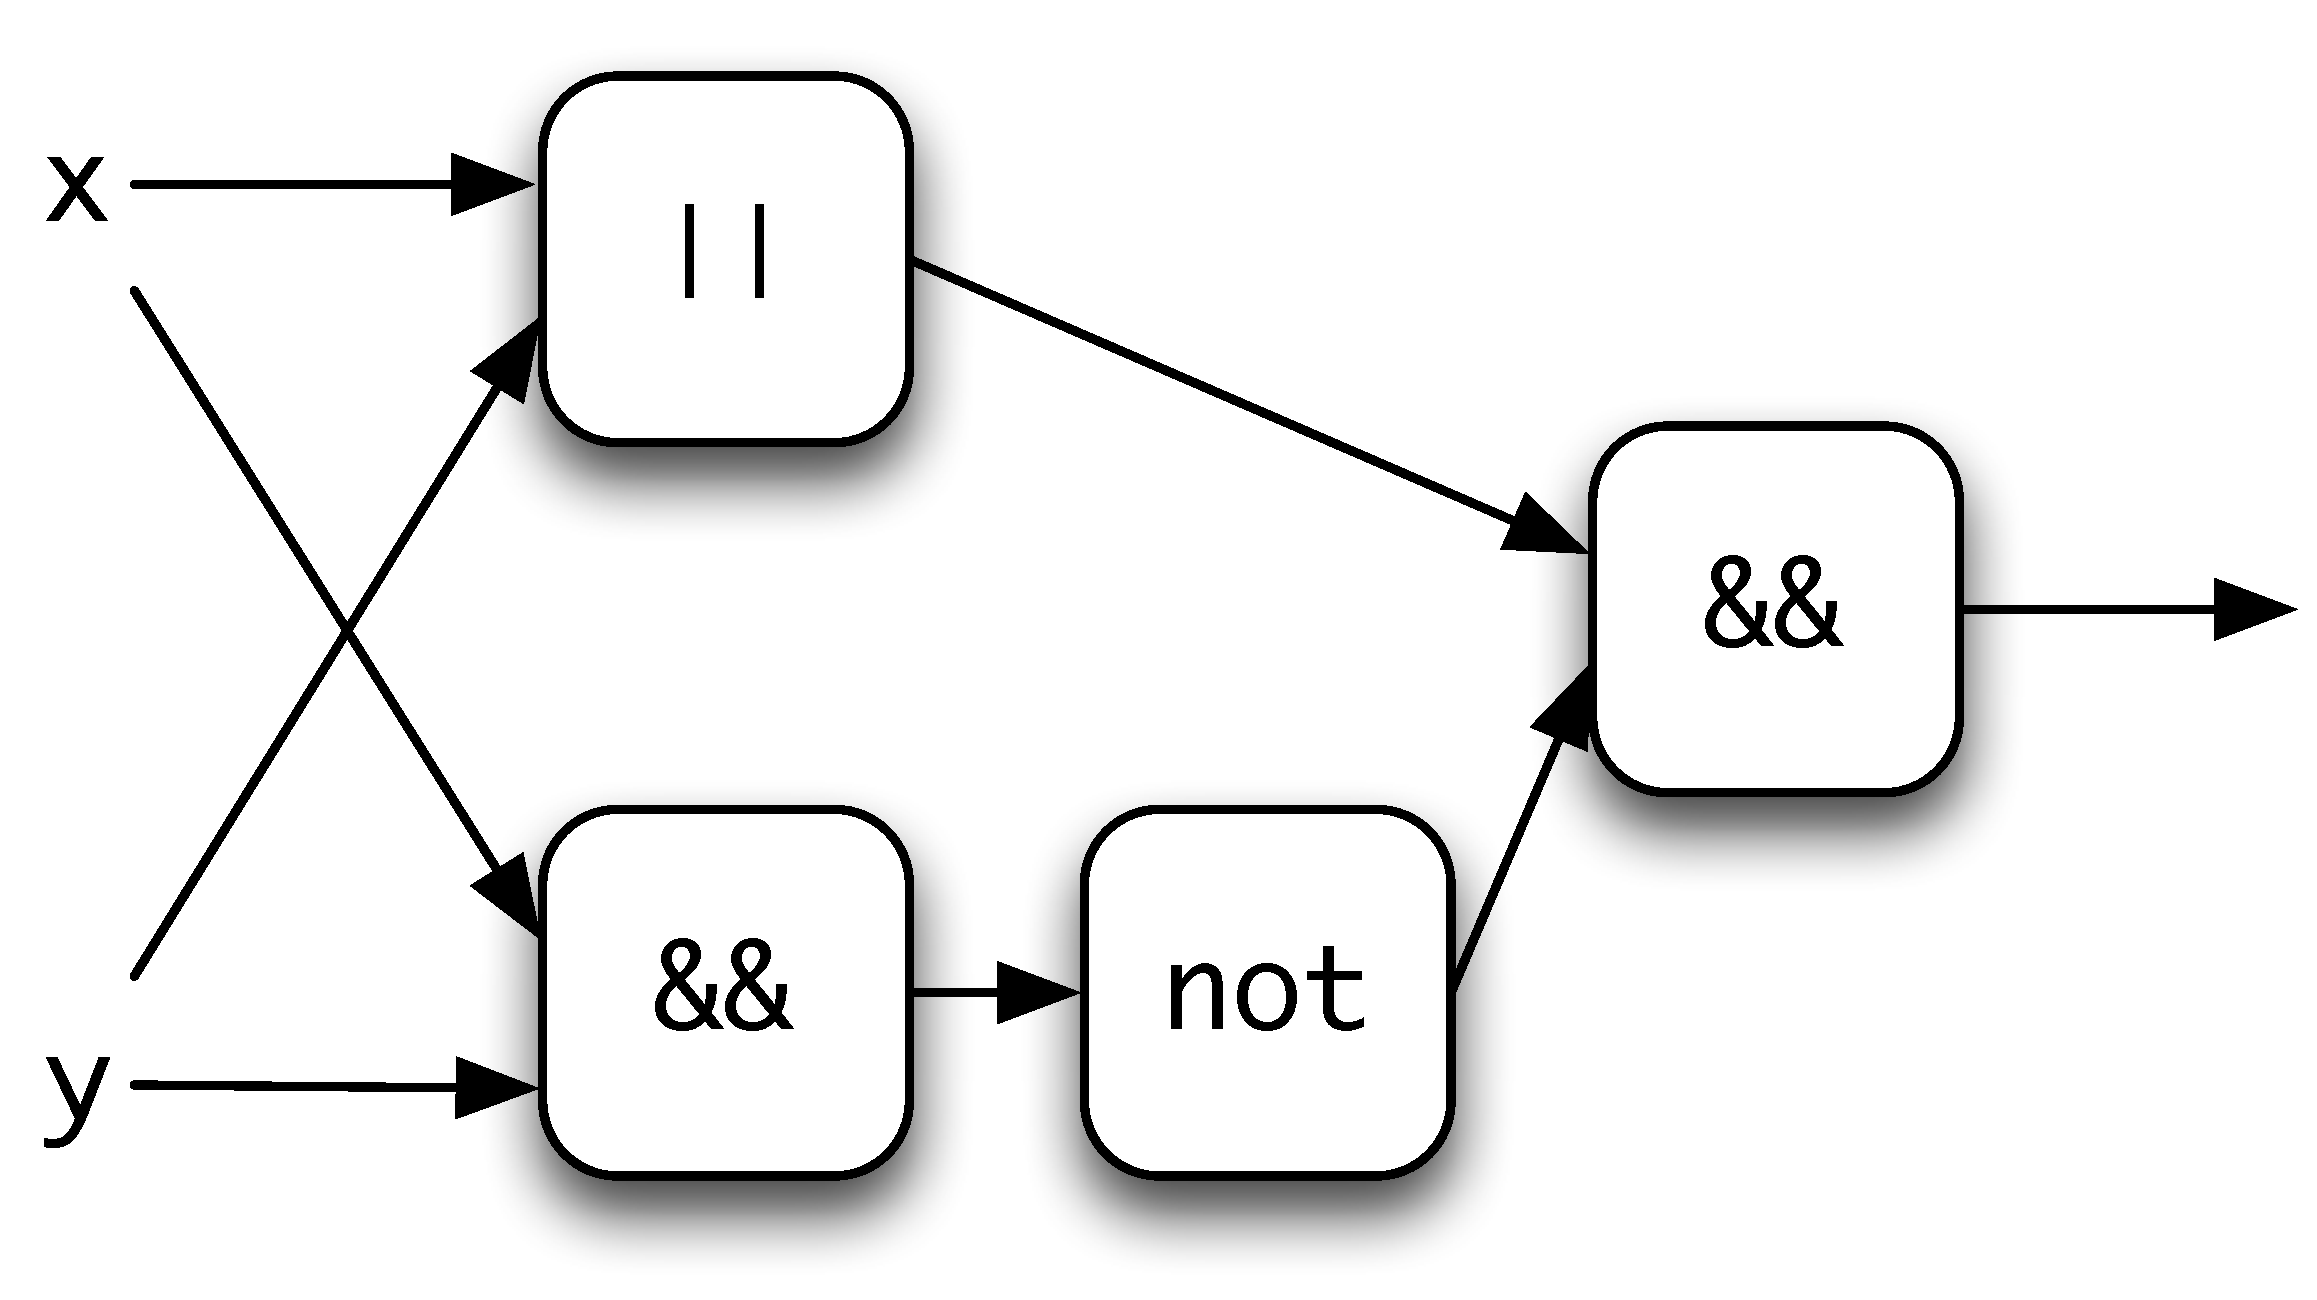
\includegraphics[height=4cm]{Pictures/exOr.pdf}
\end{center} 
Boolean values can also be compared for equality and inequality using
the operators
\texttt{==}\minx{==} and \texttt{/=}\minx{/=}, which both have the type
\begin{alltt}
Bool -> Bool -> Bool
\end{alltt}
Note that \texttt{/=} is the same function as \texttt{exOr}, since both
return the result \texttt{True} when exactly one of their arguments is
\texttt{True}.

\subsection*{Literals and definitions}

Expressions like \texttt{True} and \texttt{False}, and also numbers like
\texttt{2}, are known as
\textbf{literals}.\index{literal}\index{value!literal}
These are values which are given literally, and which need no
evaluation; the result of evaluating a literal is the literal itself.

We can use the literals \texttt{True} and \texttt{False} as arguments, in defining
\texttt{not} for ourselves:
\begin{alltt}\minx{myNot}
myNot :: Bool -> Bool
myNot True  = False
myNot False = True
\end{alltt}
We can also use a combination of literals and variables on the left-hand side of
equations defining \texttt{exOr}:
\begin{alltt}
exOr True  x = not x
exOr False x = x
\end{alltt}
Here we see a definition of a function which uses two equations: the
first applies whenever the first argument to \texttt{exOr} is
\texttt{True} and the second when that argument is \texttt{False}.

Definitions which use \texttt{True} and \texttt{False} on the left-hand
side of equations are often more readable than definitions which only
have variables on the left-hand side. This is a simple example of the
general \textbf{pattern matching}\index{pattern matching} 
mechanism in Haskell, which we look at
in detail in Chapter \ref{tupleList}.


\subsection*{Testing}

We can write some QuickCheck properties to test our new implementation of \texttt{not} and our multiple implementations of exclusive or. We test \texttt{myNot} against the built in function, and test our exclusive or functions -- let's call them \texttt{exOr} and \texttt{exOr1}:
\begin{alltt}\minx{prop\_myNot}
prop_myNot :: Bool -> Bool

prop_myNot x =
    not x == myNot x

prop_exOrs :: Bool -> Bool -> Bool

prop_exOrs x y =
    exOr x y == exOr1 x y 
\end{alltt}\minx{prop\_exOrs}
and running them gives the results that we expect:
\begin{alltt}
\textsl{*Chapter3>} quickCheck prop_myNot
\textsl{+++ OK, passed 100 tests.}
\textsl{*Chapter3>} quickCheck prop_exOrs
\textsl{+++ OK, passed 100 tests.}
\end{alltt}
We can also check the earlier assertion that \texttt{exOr} and \texttt{/=} have the same behaviour over Booleans with this property:
\begin{alltt}
prop_exOr2 :: Bool -> Bool -> Bool

prop_exOr2 x y =
    exOr x y == (x /= y)
\end{alltt}


\begin{exercises}
\item
Give another version of the definition of `exclusive or' which
works informally
like this: `exclusive or of \texttt{x} and \texttt{y} will be \texttt{True} if either
\texttt{x} is \texttt{True} and \texttt{y} is \texttt{False}, or \texttt{x} is \texttt{False} and \texttt{y} is \texttt{True}'.

\item Give the `box and line' diagram corresponding to your answer to the 
previous question.

\item Using literals on the left-hand side we can make the truth table
for a function into its Haskell definition. Complete the following
definition of \texttt{exOr} in this style.
\begin{alltt}
exOr True True  = ...
exOr True False = ...
  ...
\end{alltt}

\item Give your own definitions of the built-in \texttt{\&\&} and \texttt{||}. If you want to use the same operator for \texttt{\&\&}, say, you will need to make sure you hide its import. You can do this by adding it to the list of what is hidden, thus:
\begin{alltt}
import Prelude hiding (max,(&&))
\end{alltt}
after the \texttt{module} declaration at the start of the \texttt{Chapter3} module.

\item Give two different definitions of the \texttt{nAnd} function 
\begin{alltt}
nAnd :: Bool -> Bool -> Bool
\end{alltt}
which returns the result \texttt{True} except when both its arguments
are \texttt{True}. Give a diagram illustrating one of your definitions.

\item
Give line-by-line calculations of 
\begin{alltt}
nAnd True True
nAnd True False
\end{alltt}
for each of your definitions of \texttt{nAnd} in the previous exercise.


\item
Write QuickCheck properties to test the functions you have written in the earlier exercises. You might be able to check one version of a function against another, or perhaps think up different properties for your functions.

\index{Booleans|)}
\end{exercises}


\section{The integers: \texttt{Integer} and \texttt{Int}}
\markright{The integers: \texttt{\runinghead Integer}}
\label{ints}
\index{numbers!integers|(}\minx{Integer}

The Haskell type \texttt{Integer} contains the integers, which are the whole numbers, positive, zero and negative, used for counting; they
are written like this:

\begin{alltt}
0
45
-3452
2147483647
\end{alltt} 
Integers in the \texttt{Integer} type can be as large as you wish: looking back at the GHCi screenshots in Figures \ref{GHCiSessionMac} and \ref{WinGHCiSession} you can see examples of this. We do arithmetic on integers using the following operators and functions.

\medskip
\noindent
\begin{mytable}
\texttt{+}\minx{+} & The sum of two integers. \\
\texttt{*}\minx{*} & The product of two integers.\\
\texttt{\^{}}\minx{\^{}} & Raise to the power; \texttt{2\^{}3} is \texttt{8}.\\
\texttt{-}\minx{-} & The difference of two integers, when infix: \texttt{a-b}; 
the integer of opposite sign, when prefix: \texttt{-a}.\\ 
\texttt{div}\minx{div} & Whole number division; for example \texttt{div 14 3} is \texttt{4}. This
can also be written \texttt{14 `div` 3}.\\
\texttt{mod}\minx{mod} & The remainder from whole number division; for example \texttt{mod 14 3}
(or \texttt{14 `mod`
3}) is \texttt{2}.\\
\texttt{abs\minx{abs}} & The absolute value of an integer; remove the sign.\\
\texttt{negate\minx{negate}} & The function to change the sign of an integer.\\
\end{mytable}


\medskip
\noindent
Note that \texttt{`mod`} surrounded by \textbf{backquotes}
\index{backquote (\texttt{`})} is written between its two arguments, is
an {\bf infix}\index{function!infix version of}\index{infix version of a function} 
version of the function \texttt{mod}.
Any function can be made infix in this
way. 

In what follows we will use the term the \textbf{natural numbers} for the
\index{numbers!natural numbers}
non-negative integers: \texttt{0}, \texttt{1}, \texttt{2}, \ldots.

\begin{figure}[t]
\index{pitfalls!negative literals}\index{literal!negative}
\beware{Negative literals}{Negative literals cause problems in Haskell, because of the way that they have been defined. For example the number minus twelve is written as \texttt{-12}, but the prefix `\texttt{-}'
can often get confused with the infix operator to subtract one number from another
and can lead to unforeseen and confusing type error messages. For
example, the application
\begin{alltt}
negate -34
\end{alltt}
\noindent is interpreted as `negate minus \texttt{34}' and
leads to a GHCi error message: we discuss how to interpret that in the next note.

\medskip
\noindent
If you are in any doubt about the source of an error and you are
dealing with negative numbers you should
enclose them in parentheses, thus: \texttt{negate (-34)}; it will do no harm! See
Section \ref{operators} for more details.}
\end{figure}

\begin{figure}[t]
\beware{Understanding GHCi error messages}{When you first see an error message like this
\begin{alltt}\index{GHCi!understanding error messages}
    No instance for (Num (a -> a))
      arising from a use of `-' at <interactive>:1:0-9
    Possible fix: add an instance declaration for (Num (a -> a))
      In the expression: negate - 34
    In the definition of `it': it = negate - 34
\end{alltt}
you could be forgiven for being bemused, because it talks about things we've not covered yet. 

\medskip\noindent
Don't despair! What you can do is \textbf{extract some useful information} from it, particularly from the parts highlighted with a white background. The first one says that there's something wrong with a use of `\texttt{-}' on the line typed \emph{interactively}; the second one says it's because of the expression \texttt{negate - 34}, where you can see that the system has mis-interpreted your use of \texttt{-34}.

\medskip\noindent
So, you need to be a detective, pulling out all the \emph{clues} that you can find. These will usually be some indication of \emph{where the error occurs} and \emph{the reason for it}. If nothing else, it should give you a clue of where to look.
}
\end{figure}





\subsection*{Relational operators}

There are ordering and (in)equality\index{order}\index{equality}
relations over the integers, as there are
over all basic types. These functions
take two integers as input and return a \texttt{Bool}, that is 
either \texttt{True} or \texttt{False}. The relations are 
 
\medskip
\noindent
\begin{mytable}
\mi > & greater than (and not equal to) \minx{>}\\
\mi >= & greater than or equal to \minx{>=}\\
\mi == & equal to\minx{==} \\
\mi /= & not equal to\minx{/=}\\
\mi <= & less than or equal to\minx{<=}\\
\mi < & less than (and not equal to)\minx{<}
\end{mytable}


\medskip
\noindent
A simple example using these definitions is a function to test whether
three \texttt{Integer}s are equal.
\begin{alltt}\minx{threeEqual}
threeEqual :: Integer -> Integer -> Integer -> Bool
threeEqual m n p = (m==n) \&\& (n==p)
\end{alltt}
%\vspace{-5pt}


\begin{figure}[t]
\beware{Fixed-size integers: the \texttt{Int} type}{\minx{Int}
The \texttt{Int} type represents integers in a fixed amount of space, and
so can only represent a finite range of integers. The value
\texttt{maxBound} gives the greatest value in the type, which happens to be
\texttt{2147483647}. 

\medskip
\noindent
For many integer
calculations these fixed size numbers are suitable, and they have the advantage of being more efficient, but if larger
numbers may be 
required it's better to use the \texttt{Integer}\minx{Integer} type, which can accurately represent whole numbers of
any size. 

\medskip
\noindent
The reason that we introduce \texttt{Int} at all is that because some of the standard Haskell functions
which we introduce later in the chapter use the \texttt{Int} type, rather than \texttt{Integer}.

\medskip
\noindent
What functions and operators can we use over \texttt{Int}? All the functions we have already given for \texttt{Integer}, in fact, because these functions are \emph{overloaded}: we look at this in Section \ref{overlIntro}. We can also covert between the two types using
\begin{alltt}\minx{fromInteger}\index{toInteger}
fromInteger :: Integer -> Int
toInteger   :: Int -> Integer
\end{alltt}}
\end{figure}


\begin{exercises}
\vspace{-3pt}
\item
Explain the effect of the function defined here:
\begin{alltt}
mystery :: Integer -> Integer -> Integer -> Bool
mystery m n p = not ((m==n) \&\& (n==p))
\end{alltt}
Hint: if you find it difficult to answer this question directly, try to
see what the function does on some example inputs.

\item
Define a function 
\begin{alltt}
threeDifferent :: Integer -> Integer -> Integer -> Bool
\end{alltt}
so that the result of \texttt{threeDifferent m n p} is \texttt{True}
only if all three of the numbers \texttt{m}, \texttt{n} and \texttt{p}
are different.

What is your answer for \texttt{threeDifferent 3 4 3}? Explain why you
get the answer that you do.

\item
This question is about the function
\begin{alltt}
fourEqual :: Integer -> Integer -> Integer -> Integer -> Bool
\end{alltt}
which returns the value \texttt{True} only if all four of its arguments
are equal.

Give a definition of \texttt{fourEqual} modelled on the
definition of \texttt{threeEqual} above. Now give a definition of
\texttt{fourEqual} which {\em uses\/} the function \texttt{threeEqual}
in its definition. Compare your two answers.

\item
Give line-by-line calculations of
\begin{alltt}
threeEqual (2+3) 5 (11 `div` 2)
mystery (2+4) 5 (11 `div` 2)
threeDifferent (2+4) 5 (11 `div` 2)
fourEqual (2+3) 5 (11 `div` 2) (21 `mod` 11)
\end{alltt}

\item
Devise QuickCheck tests for the functions that you have defined here.



\index{numbers!integers|)}%
\end{exercises}
\vspace{-20pt}

\section{Overloading}
\label{overlIntro}
\index{overloading}%
\index{name!overloading of}%

\texttt{Integer}s, \texttt{Int}s and Booleans can all compared for equality, and the same
symbol \texttt{==} is used for all these operations, even though they
are different. Indeed, \texttt{==} will be used for equality over
any type \texttt{t} for which we are able to define an equality
operator. This means that \texttt{(==)} will have the type 
\begin{alltt}\minx{==}
Int -> Int -> Bool
Integer -> Integer  -> Bool
Bool -> Bool -> Bool
\end{alltt}
and indeed \texttt{t -> t -> Bool} if the type \texttt{t}
carries an equality.

Using the same symbol or name for different operations is called
\textbf{overloading}. A number of symbols in Haskell are overloaded, and
we will see in Chapter \ref{typeClasses} how overloading is handled in the
type system of Haskell, and also how users can define their own
overloaded operators or names.

\beware{The type for equality}{The type for equality, \texttt{t -> t -> Bool} for any type \texttt{t} carrying an equality, \emph{doesn't} allow us to compare elements from different types for equality. So, if we evaluate\index{equality!type of}
\begin{alltt}
2 == True
\end{alltt}
we get an error message from GHCi. Of course, there's not much point in comparing values of different types, because they will never be equal! We'll come back to this in Chapter \ref{typeClasses}.
}

\section{Guards}
\label{guards}
\index{guard|(}
\index{Boolean!guard|see{guard}}

Here we explore how conditions or \textbf{guards} are used to give
alternatives in the definitions of functions. A guard is a Boolean expression, and
these expressions are used to express various cases in the definition of a function.
 
We take as a running
example in this section
functions which compare integers for size, and start by looking
at the example of the function to return the maximum value of two
integers. When the two numbers are the same then we call their common value
the maximum.
\begin{alltt}\minx{max}
max :: Integer -> Integer -> Integer
max x y
  | x >= y      = x
  | otherwise   = y
\end{alltt}
How do we read a definition like this, which appears in the Haskell prelude? 
%\psdraft
\begin{center}
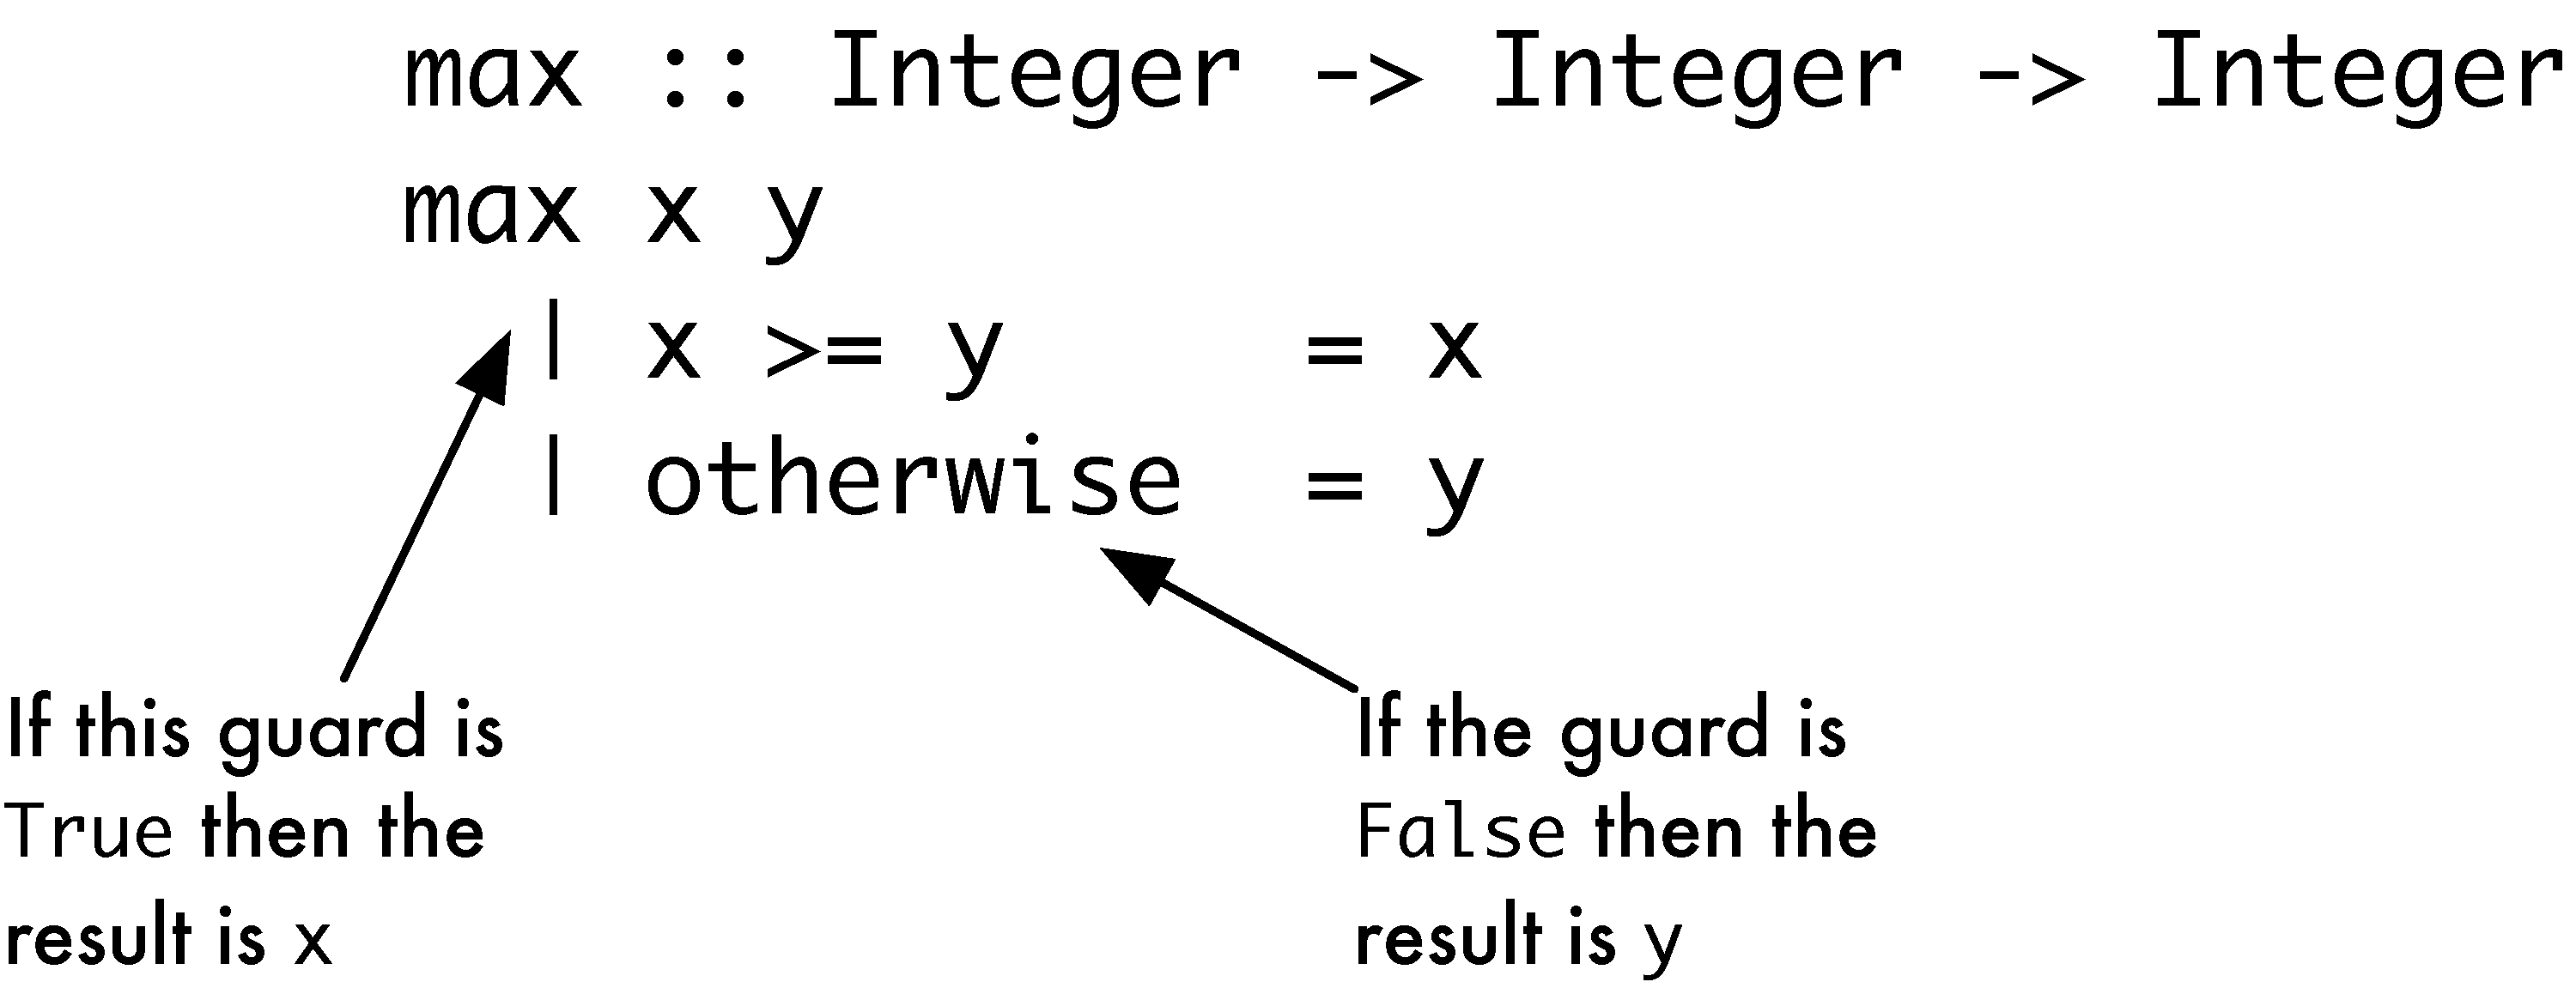
\includegraphics[width=4in]{Pictures/max.pdf}
\end{center} 
%\psfull
In general, if the first guard (here \texttt{x>=y})
is \texttt{True} then the corresponding value is the result (\texttt{x} in this case).
On the other hand, if the first guard is \texttt{False}, then we look at the second, and so on. 
An \texttt{otherwise}\minx{otherwise}
guard will hold whatever the arguments, so that in the case of \texttt{max} the result is \texttt{x} if 
\texttt{x>=y} and \texttt{y} otherwise, that is in the case that \texttt{y>x}.

 
An example in which there are multiple guards is a definition of the
maximum of three inputs.
\begin{alltt}\minx{maxThree}
maxThree :: Integer -> Integer -> Integer -> Integer
maxThree x y z
  | x >= y \&\& x >= z    = x
  | y >= z              = y
  | otherwise           = z
\end{alltt}
How does this definition work? The first guard
\begin{alltt}
x >= y \&\& x >= z
\end{alltt}
tests whether \texttt{x} is the maximum of the three inputs; if it is \texttt{True}
the corresponding result is \texttt{x}. If the guard fails, then \texttt{x} is
not the maximum, so there has to be a choice between \texttt{y} and \texttt{z}. The
second guard is therefore
\begin{alltt}
y >= z
\end{alltt}
If this holds, the result is \texttt{y}; otherwise the result is
\texttt{z}. We will go back to the example of \texttt{maxThree} in Section
\ref{probSolvIntro}.

We first gave a general form for simple function definitions in Chapter
\ref{intro}; we can now strengthen this to give a general form for
function definitions with guards in Figure \ref{funGuardDef}. Note that
the \texttt{otherwise} is not compulsory.
\index{function definition!general form}

%fig3.1
\begin{figure}
\begin{center}
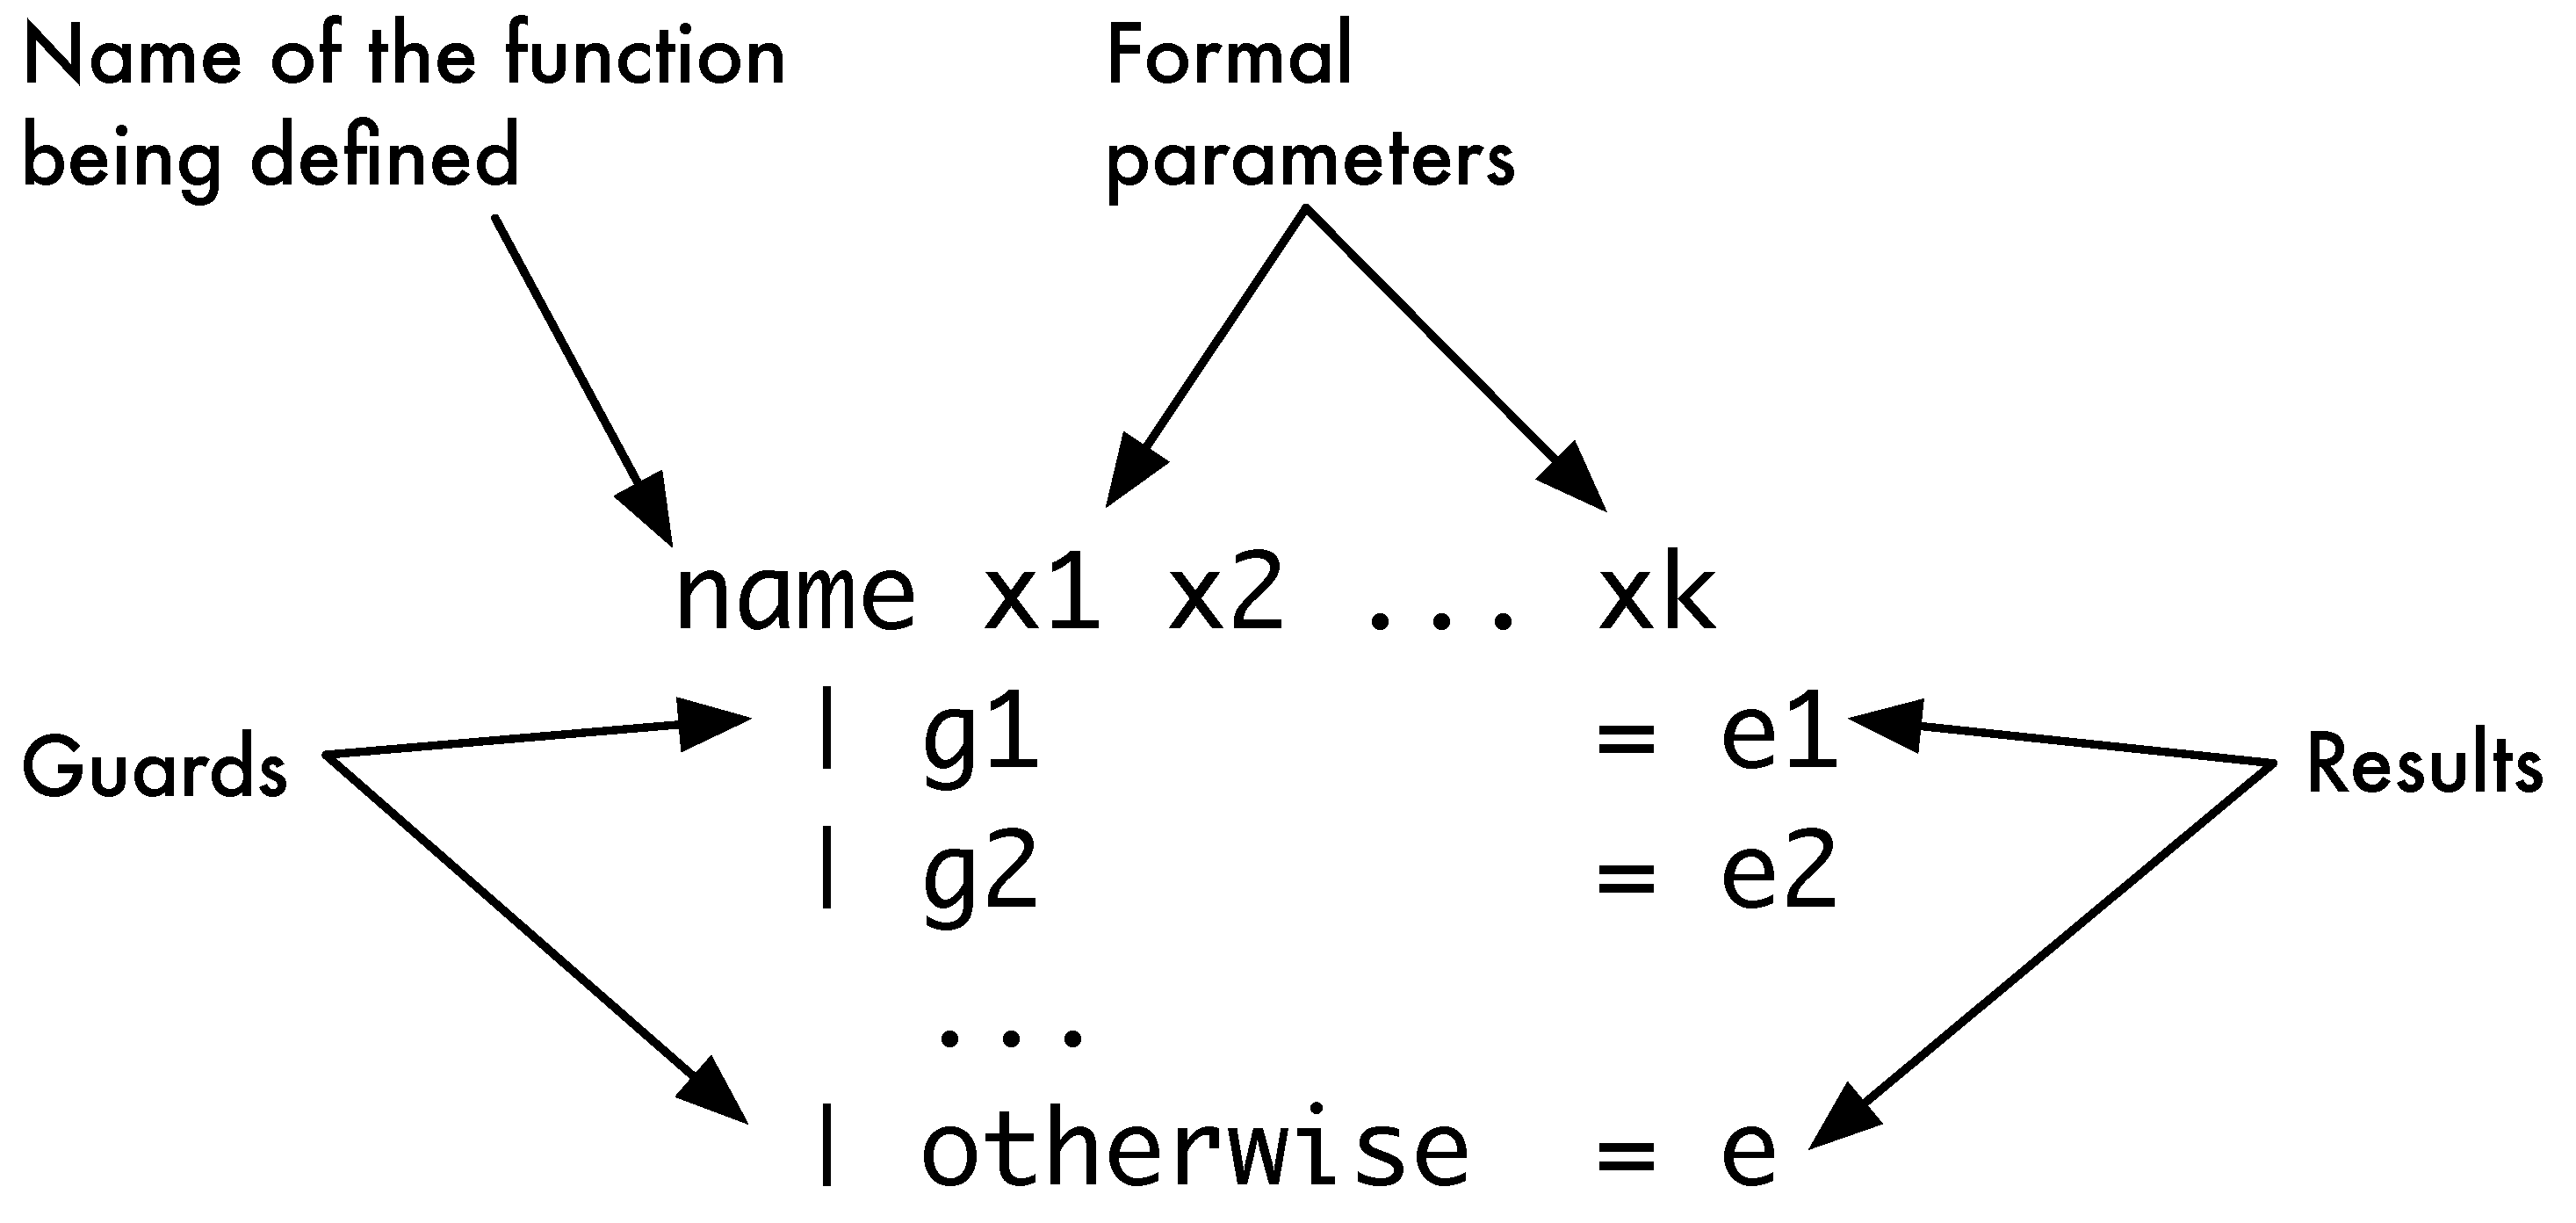
\includegraphics[width=4in]{Pictures/funGuardDef.pdf}
\end{center} 
\caption{The general form for function definitions with guards.}
\label{funGuardDef}
\end{figure}

We also saw in Chapter \ref{intro} that we can write down line-by-line
\textbf{calculations}\index{calculation!guards}
of the values of expressions. How do guards fit into this model? When we
apply a function to its arguments we need to know which of the cases
applies, and to do this we need to evaluate the guards until we find a
guard whose value is \texttt{True}; once we find this, we can evaluate
the corresponding result. Taking the example of \texttt{maxThree}, we
give two examples in which we perform the evaluation of guards on lines
beginning `\texttt{??}'.
\begin{alltt}
maxThree 4 3 2
  ?? 4>=3 \&\& 4>=2
  ?? \step{}True \&\& True
  ?? \step{}True
\step{}4
\end{alltt}
In this example the first guard we try, \texttt{4>=3 \&\& 4>=2},
gives \texttt{True} and so the result is the corresponding value,
\texttt{4}.
In the second example we have to evaluate more than one guard.
\begin{alltt}
maxThree 6 (4+3) 5
  ?? 6>=(4+3) \&\& 6>=5
  ?? \step{}6>=7 \&\& 6>=5
  ?? \step{}False \&\& True
  ?? \step{}False
  ?? 7>=5
  ?? \step{}True
\step{}7
\end{alltt}
In this example we first evaluate the first guard, \texttt{6>=(4+3) \&\&
6>=5}, which results in \texttt{False}; we therefore evaluate the
second guard, \texttt{7>=5}, which gives \texttt{True}, and so the
result is \texttt{7}. 

Once we have calculated the value of the second
argument, \texttt{(4+3)}, we do not re-calculate its value when we
look at it again. This is not just a trick on our part; the GHCi system will only 
evaluate an argument like \texttt{(4+3)} 
once, keeping its value in case it is needed again, as indeed it is in
this calculation. This is one aspect of lazy evaluation, which is the
topic of Chapter \ref{lazy}.

\subsection*{Conditional expressions}
\index{conditional expression}\index{expression!conditional}
\index{Boolean!conditional expression}
\index{if@{\texttt{if}\ldots\texttt{then}\ldots\texttt{else}}}

Guards are conditions which distinguish between
different cases in definitions\break of functions. We
can also write general conditional expressions by means of
the\break{\texttt{if}\ldots\texttt{then}\ldots\texttt{else}} construct of Haskell. The value of
\begin{alltt}
if condition then m else n
\end{alltt}
is \texttt{m} if the \texttt{condition} is \texttt{True} and is
\texttt{n} if the \texttt{condition} is \texttt{False}, so that the
expression \texttt{if False then 3 else 4}
has the value \texttt{4}, and in general
\begin{alltt}
if x >= y then x else y
\end{alltt}
will be the maximum of \texttt{x}
and \texttt{y}. This shows that we can write \texttt{max'} in a
different way thus:
\begin{alltt}
max' :: Integer -> Integer -> Integer
max' x yMax
  = if x >= y then x else y
\end{alltt}
We tend to use the guard form rather than this, but we will see examples
below where the use of \texttt{if ...\ then ...\ else ...{}} is more
natural.

\subsection*{Testing}

We can test our implementations of `maximum' by checking that they have the same behaviour, as we did earlier, writing a QuickCheck property like this:
\begin{alltt}\minx{prop\_compareMax}
prop_compareMax :: Integer -> Integer -> Bool
prop_compareMax x y =
    max x y == max' x y
\end{alltt}
But this is not the only way of writing properties. We can often write down a collection of properties which together say what a function should do. In the case of \texttt{max} we can say two things
\begin{itemize}
\item
The maximum of \texttt{x} and \texttt{y} will be greater than or equal to both \texttt{x} and \texttt{y}.
\item
The maximum of \texttt{x} and \texttt{y} will actually be equal to one (or both) of  \texttt{x} and \texttt{y}.
\end{itemize}  
We can write these two as QuickCheck properties, 
\begin{alltt}
prop_max1, prop_max2 :: Integer -> Integer -> Bool

prop_max1 x y =
    x <= max x y && y <= max x y

prop_max2 x y =
    x == max x y || y == max x y
\end{alltt}
and check whether they hold. 

\begin{figure}[t]
\beware{Properties can be wrong too}{\index{property!incorrect}
Sometimes we make mistakes writing properties. Suppose we'd written the property 
\texttt{prop\_max2} like this instead:
\begin{alltt}
prop\_max3 x y =

\ \ \ \ (x == max x y) `exOr` (y == max x y)
\end{alltt}
recall that QuickCheck will give us a \emph{counterexample}, that is, an example of where the test fails:   
\begin{alltt}
\textsl{*Chapter3>} quickCheck prop\_max3

\textsl{*** Failed! Falsifiable (after 1 test):} 
 
\textsl{0}

\textsl{0}
\end{alltt}
The example shows that the property fails when the two arguments are the same. 
That's the fault of the property, as we'd forgotten about this particular case. 
So, \textbf{when a property fails, we need to look both at the functions it is meant to test, 
and at the property itself}.}
\end{figure}


\begin{figure}[t]
\beware{Redefining prelude functions}{\label{redefName}%
The \texttt{max} function is defined in the prelude,
\texttt{Prelude.hs},\index{prelude, redefining functions in}
\index{function definition!redefining prelude functions}
and if a definition 
\begin{alltt}
max :: Integer -> Integer -> Integer
\end{alltt}
\noindent appears in a script then this definition will conflict with
the prelude definition, leading to a GHCi error messages like this
\begin{alltt}
\ \ \ \ Ambiguous occurrence `max'

\ \ \ \ It could refer to either `Chapter3.max', defined at ...

\ \ \ \ \ \ \ \ \ \ \ \ \ \ \ \ \ \ \ \ \ \ or `Prelude.max', imported from Prelude ...
\end{alltt}
\noindent To redefine the prelude functions \texttt{max} and \texttt{min}, say, the line
\begin{alltt}
import Prelude hiding (max,min)\minx{import}\minx{hiding}
\end{alltt}
\noindent which overrides the usual import of the prelude should be included at
the top of the module, after its \texttt{module}
statement.

Many of the functions defined in this text are in fact included in the
prelude, and so this technique needs to be used whenever you want to 
redefine one of these.
}\end{figure}

\begin{exercises}
\item
Give calculations of 
\begin{alltt}
max (3-2) (3*8)
maxThree (4+5) (2*6) (100 `div` 7)
\end{alltt}

\item
Give definitions of the functions
\begin{alltt}
min      :: Int -> Int -> Int
minThree :: Int -> Int -> Int -> Int
\end{alltt}
which calculate the minimum of two and three integers, respectively.

\item
Define QuickCheck properties to test the functions \texttt{maxThree}, \texttt{min} and \texttt{minThree}.


\index{guard|)}
\end{exercises}
\section{Characters and strings}
\markright{The characters: \texttt{\runinghead Char}}
\label{char}
\index{characters|(}
\minx{Char}
People and computers communicate using keyboard input and screen output,
which are based on sequences of {\bf characters}, that is letters, digits
and `special' characters like space, tab, newline and end-of-file. Haskell
\index{characters!tab}
\index{characters!end-of-file}
contains a built-in type of characters, called \texttt{Char}.\minx{Char} Sequences  or \textbf{strings} of characters form the Haskell \texttt{String} type. 

\subsection*{Characters: \texttt{Char}}

Literal characters\index{characters!literal} 
are written inside single quotes, thus {\mi 'd'} is
the Haskell representative of the character d. Similarly {\mi '3'}
is the character three. Some special characters are represented as 
follows

\medskip
\noindent
\begin{mytable}
tab & \texttt{'\bs{t}'}\\[3pt]\index{tab (\texttt{\bs{}t})}  
newline & \texttt{'\bs{n}'}\\[3pt]\index{newline (\texttt{\bs{}n})}
backslash (\verb+\+) & \texttt{'\bs{\symbol{92}}'}\\[3pt]\index{backslash (\texttt{\bs{}\bs{}})}
single quote (\texttt{'}) & \texttt{'\bs{'}'}\\[3pt]\index{single quote (\texttt{\bs{}'})}
double quote (\texttt{"}) & \texttt{'\bs{"}'}\\[3pt]\index{double quote (\texttt{\bs{\symbol{34}}})}
\end{mytable} 

\medskip
\noindent
There is a standard coding for characters as integers, called the ASCII
\index{characters!ASCII coding}
coding. The capital letters \texttt{'A'} to \texttt{'Z'} have the sequence of
codes from \texttt{65} to \texttt{90}, and the small letters \texttt{'a'} to 
\texttt{'z'} the codes \texttt{97} to \texttt{122}. The character with code \texttt{34}, for
example, can be written \texttt{'\bs{34}'}, and \texttt{'9'} and \texttt{'\bs{57}'} have the same
meaning. ASCII has recently been extended to
the Unicode\index{characters!Unicode}\index{Unicode} standard, which contains characters from other character sets
than English.

There are conversion functions between characters and their numerical
codes
which convert an integer into a character, and vice versa. 
\vspace{2pt}

\begin{alltt}
fromEnum :: Char -> Int\minx{fromEnum}
toEnum :: Int -> Char\minx{toEnum}
\end{alltt} 
\vspace{2pt}

\noindent The coding functions can be used in defining functions over
\texttt{Char}. To convert a small letter to a capital an offset needs to be
added to its code:
\vspace{2pt}

\begin{alltt}
offset :: Int
offset = fromEnum 'A' - fromEnum 'a'
 
toUpper :: Char -> Char\minx{toUpper}
toUpper ch = toEnum (fromEnum ch + offset)
\end{alltt}
\vspace{2pt}

\noindent Note that the \texttt{offset} is named, rather than appearing as a
part of
\texttt{toUpper}, as in
\vspace{2pt}

\begin{alltt}
toUpper ch = toEnum (fromEnum ch + (fromEnum 'A' - fromEnum 'a'))
\end{alltt} 
\vspace{2pt}

\noindent This is standard
practice, making the program both easier to read
and to modify. To change the offset value, we just need to
change the definition of \texttt{offset}, rather than having to change the
function (or functions) which use it.
 
Characters can be compared using
the ordering given by their codes. So, since the digits \texttt{0} to \texttt{9} occupy
a block of adjacent codes \texttt{48} to \texttt{57}, we can check whether a character 
is a digit thus:
\vspace{2pt}

\begin{alltt}\minx{isDigit}
isDigit :: Char -> Bool
isDigit ch = ('0' <= ch) \&\& (ch <= '9')
\end{alltt}
\vspace{2pt}


\noindent The standard library \texttt{Data.Char} contains a number of conversion functions like
\texttt{toUpper}, and discrimination
functions like \texttt{isDigit}.\minx{Data.Char}


\begin{exercises}

\item Define a function to convert small letters to capitals which returns
unchanged characters which are not small letters.

\item Define the function
\begin{alltt}
charToNum :: Char -> Int
\end{alltt}
which converts a digit like \texttt{'8'} to its value, \texttt{8}. The value of
non-digits should be taken to be \texttt{0}.


\end{exercises}

\index{characters|)}

\subsection*{Strings: \texttt{String}}\minx{String}

The \texttt{String} type is made up of sequences of characters, written between double quotes like this: \texttt{"This is a string!"}. In the last section 
 we showed how to write
the special characters such as newline and tab using the `escapes'
\texttt{'\bs{n}'} and \texttt{'\bs{t}'}. These characters can form part
of strings, as in the examples
\begin{alltt}
"baboon"
""
"\bs{9}9a\bs{1}16"
"gorilla\bs{n}hippo\bs{n}ibex"
"1\bs{t}23\bs{t}456"
\end{alltt}
If we evaluate one of these strings in GHCi, the result is exactly the same as the
input. In order to resolve the escape characters  and to lose the double quotes we have to
perform an output operation. This is done using the primitive Haskell function
\begin{alltt}\minx{putStr}
putStr :: String -> IO ()
\end{alltt} 
with the effect of putting the argument string on the screen. Applying \texttt{putStr} 
to each of the strings above gives output as follows:
\begin{alltt}
baboon

cat
gorilla
hippo
ibex
1       23      456
\end{alltt}
Strings can be joined together using \texttt{++}\minx{++}, so that 
\texttt{"cat"++"\bs{n}"++"fish"} prints as
\begin{alltt}
cat
fish
\end{alltt}

We'll cover strings in more detail -- in particular seeing how we can write functions to create and manipulate strings -- in Chapter \ref{tupleList} below. 

\begin{figure}[t]\index{name!and strings and characters}
\beware{Names, strings and characters}{\index{pitfalls!\texttt{Char} and \texttt{String}}
It is easy to confuse \texttt{a}, \texttt{'a'} and \texttt{"a"}. To summarize
the difference,

\medskip
\noindent
\begin{mytable}
\mi a & is a name or a variable, if defined it may have any type whatever;\\  
\mi 'a'  & is a character, so of type \texttt{Char};\\
\mi "a"  & is a string, and of type \texttt{String}, which just happens to consist of a single character.
\end{mytable}

\medskip
\noindent
Similarly, there is a difference between

\medskip
\noindent
\begin{mytable}
\mi emu & a Haskell name or variable;\\
\mi "emu" & a string of type \texttt{String}.
\end{mytable} 
}\end{figure}


\subsection*{Strings and values}

Built into Haskell are the overloaded functions \texttt{show}\index{show@\texttt{show}}
and \texttt{read}\minx{read}, which convert from a value to a
\texttt{String} and
vice versa; for instance,
\begin{alltt}
show (2+3)           \step{}"5"
show (True || False) \step{}"True"
\end{alltt}
In the opposite direction, the function \texttt{read} is used to convert
a string to the value it represents, so that
\begin{alltt}
read "True" \step{}True
read "3"    \step{}3
\end{alltt}
In some situations it will not be clear what should be the result type
for
\texttt{read} -- it is then possible to give a type to the application,
as in
\begin{alltt}
(read "3") :: Int
\end{alltt}
the  result of which will be \texttt{3} and its type, \texttt{Int}. 
A
full explanation of the types of \texttt{read} and \texttt{show} can be
found in Chapter \ref{typeClasses}.











\begin{exercises}

\item Define a function 
\begin{alltt}
onThreeLines :: String -> String -> String -> String
\end{alltt}
which takes three strings and returns a single string which when printed
shows the three strings on separate lines.


\item Define a function
\begin{alltt}
romanDigit :: Char -> String
\end{alltt}
which converts a digit to its representation in Roman numerals, so 
at \texttt{'7'} it will have the value \texttt{"VII"} and so on.

\end{exercises}



\section{Floating-point numbers: \texttt{Float}}
\markright{Floating-point numbers: \texttt{\runinghead Float}}
\label{float}
\index{numbers!floating point|(}
\minx{Float}\minx{Double}

In Section \ref{ints} we introduced the Haskell type \texttt{Int} of integers.
In calculating we also want to use numbers with fractional parts, which
are represented in Haskell by the \textbf{floating-point} numbers which
make up the type \texttt{Float}. We do not use \texttt{Float} heavily in
what follows, and so this section can be omitted on first reading and
used as reference material to be consulted when necessary.

Internal to the Haskell system there is a fixed amount of space allocated to
representing each \texttt{Float}. This has the effect that
not all fractions can be
represented by floating-point numbers, and
arithmetic over them will not always be exact. It is possible to use the
type of double-precision floating-point numbers, \texttt{Double}\minx{Double} for greater
precision, or for full-precision fractions built from \texttt{Integer} there is the
type \texttt{Rational}. As 
this is a
programming tutorial we restrict our attention to the types \texttt{Int} and 
\texttt{Float} but we shall survey the numerical types briefly in Chapter
\ref{typeClasses}.

Literal floats in
Haskell can be given by decimal numerals, such as
\begin{alltt}
0.31426
-23.12
567.347
4523.0
\end{alltt}
The numbers are
called floating point because the position of the decimal point is not the
same for all \texttt{Floats};
depending upon the particular number, more of the space can be used to store
the integer or the fractional part.

\begin{figure}[t]\minx{+}\minx{-}\minx{*}\minx{**}
\noindent\begin{tabular}{p{1.0in}p{1.9in}p{1.9in}}
\ttfamily + - * & \ttfamily Float -> Float -> Float & Add, subtract, multiply.\\
\ttfamily /\minx{/} & \ttfamily Float -> Float -> Float & Fractional division. \\
\ttfamily \^{}\minx{\^{}} & \ttfamily Float -> Integer -> Float & Exponentiation \texttt{x\^{}n = \superscr{x}{n}} for a natural number \texttt{n}.\\
\ttfamily ** & \ttfamily Float -> Float -> Float & Exponentiation \texttt{x**y = \superscr{x}{y}}.\\
\ttfamily ==,/=,<,>, & \ttfamily Float -> Float -> Bool & Equality and ordering operations.\\
\ttfamily \ <=,>= & & \\
\ttfamily abs & \ttfamily Float -> Float & Absolute value.\\
\ttfamily acos,asin & \ttfamily Float -> Float & The inverse of cosine, sine\\
\ttfamily \ atan & & and tangent.\\
\ttfamily ceiling & \ttfamily Float -> Integer & Convert a fraction to an integer \\
\ttfamily \ floor & & by rounding up, down, or to the \\
\ttfamily \ round & & closest integer.\\
\ttfamily cos,sin& \ttfamily Float -> Float &  Cosine, sine and tangent.\\
\ttfamily \ tan& & \\
\ttfamily exp & \ttfamily Float -> Float & Powers of e. \\
\ttfamily fromInteger  & \ttfamily Integer -> Float & Convert an \texttt{Integer} to a \texttt{Float}.\minx{fromInteger} \\
\ttfamily fromIntegral & \ttfamily Int -> Float & Convert an \texttt{Int} (or any integral value) to a \texttt{Float}.\minx{fromIntegral} \\
\ttfamily log & \ttfamily Float -> Float & Logarithm to base e.\\
\ttfamily logBase & \ttfamily Float -> Float -> Float & Logarithm to arbitrary base, provided as first argument.\\
\ttfamily negate & \ttfamily Float -> Float & Change the sign of a number. \\
%\ttfamily read & \ttfamily String -> Float & Converts a string representing a \texttt{Float} to its value.  \minx{read}\\
\ttfamily pi & \ttfamily Float & The constant pi.\\
%\ttfamily show & \ttfamily Float -> String & Convert a number to a string. \minx{show}\\
\ttfamily signum & \ttfamily Float -> Float & \texttt{1.0}, \texttt{0.0} or \texttt{-1.0} according to whether the argument is positive, zero or negative.\minx{signum}\\
\ttfamily sqrt & \ttfamily Float -> Float & (Positive) square root. \minx{sqrt}
\end{tabular}
\caption{Floating-point operations and functions.}
\label{numOps}
\index{operator!floating point}
\index{floating point operators}
\end{figure}


Haskell also allows literal floating-point numbers in \textbf{scientific notation}. 
\index{numbers!scientific notation}
These take the form
below, where their values are given in the right-hand column of the table

\medskip
\noindent
\begin{mytable}
\texttt{231.61e7}  &\mbox{\(231.61\times{}10^7\hskip6pt= 2,316,100,000\)}\\
\texttt{231.6e-2}  &\mbox{\(231.61\times{}10^{-2} = 2.3161\)} \\
\texttt{-3.412e03} &\mbox{\(-3.412\times{}10^3\hskip3pt= -3412\)} 
\end{mytable}

\medskip
\noindent
This representation is more convenient than the decimal numerals above 
for very large and small numbers.
Consider the number \texttt{\superscr{2.1}{444}}. This will need well over
a hundred digits before the decimal point, and this would not be possible in
decimal notation of limited size (usually 20 digits at most). In scientific
notation, it will be written as \inso\mbox{}1.162433e+143\inst.

%fig3.2





\begin{figure}[t]
\beware{Non-numerical results}{\index{numbers!non-numerical results}
Some calculations over floating point numbers don't give numerical results. These could be signalled in a variety of ways; Haskell will return an indication that the result is `not a number', \texttt{NaN},\minx{NaN} or infinite, \texttt{Infinity}.\minx{Infinity} These give an indication of what has gone wrong, but can't be used in further calculations: once a value is `not a number' any calculation with it will have the same result.}\end{figure}

\medskip
\noindent
Haskell provides a range of operators and functions over \texttt{Float} in the
standard prelude. The table in Figure \ref{numOps} gives their name, type
and a brief description of their behaviour. Included are the 
\begin{titemize}
\item standard
mathematical operations: square root,
exponential, logarithm and trigonometric functions;
%\item printing and reading functions: \texttt{show}\minx{show},
%\texttt{read}\minx{read}; 
\item functions to convert integers to floating-point numbers: \texttt{fromInt},
and vice versa: \texttt{ceiling}, \texttt{floor} and \texttt{round}.
\end{titemize} 
Haskell can be used as a numeric calculator. Try typing the expression
which follows to the GHCi prompt:
\begin{alltt}
sin (pi/4) * sqrt 2
\end{alltt}

\begin{figure}[t]
\beware{Converting integers to floating-point numbers}{\index{pitfalls!numeric conversions}%
Although literals are overloaded, there is no automatic conversion from
\texttt{Integer} to \texttt{Float}.\index{numbers!conversion between types}
In general if we wish to add an integer quantity, like \texttt{floor 5.6},
to a float, like \texttt{6.7}, we will receive an error message if we type
\begin{alltt}
(floor 5.6) + 6.7
\end{alltt}
since we are trying to add quantities of two different types. We have
to convert the \texttt{Integer} to a \texttt{Float} to perform the addition, thus:
\begin{alltt}
fromIntegral (floor 5.6) + 6.7\end{alltt}
where \texttt{fromIntegral}\minx{fromIntegral}
takes anything of integral type (that is \texttt{Int}, \texttt{Integer} etc.) to the corresponding \texttt{Float}.
}\end{figure}



\subsection*{Overloaded literals and functions}

In Haskell the numbers \texttt{4} and \texttt{2}
belong to both 
\texttt{Int} and \texttt{Float}; they are overloaded, as discussed in
Section \ref{overlIntro}.  This is
\index{overloading!literals}\index{literal!overloaded}
also true of some of the numeric functions; addition, for instance, has both
the types
\begin{alltt}
Int -> Int -> Int
Float -> Float -> Float
\end{alltt}
and the relational operators \texttt{==} and so forth are available over
all basic types.
We shall explore this idea of overloading in more detail
when we discuss type classes below in Chapter \ref{typeClasses}.



\begin{exercises}
\item
Give a function to return the average of three integers
\begin{alltt}
averageThree :: Integer -> Integer -> Integer -> Float
\end{alltt}
Using this function define a function
\begin{alltt}
howManyAboveAverage :: Integer -> Integer -> Integer -> Integer
\end{alltt}
which returns how many
of its inputs are larger than their average value.

\item
How would you write QuickCheck properties to test the functions \texttt{averageThree} and \texttt{howManyAboveAverage}?

\end{exercises}

\medskip
\noindent
\label{quadratics}
The remainder of the questions look at solutions to a
\index{quadratic equation}quadratic equation
\begin{alltt}
a*\superscr{X}{2} + b*X + c = 0.0
\end{alltt}
where \texttt{a}, \texttt{b} and \texttt{c} are real numbers.
The equation has 
\begin{titemize}
\item two real roots, if {\mi \superscr{b}{2} > 4.0*a*c};
\item one real root, if {\mi \superscr{b}{2} == 4.0*a*c}; and
\item no real roots, if {\mi \superscr{b}{2} < 4.0*a*c}.
\end{titemize}
This assumes that {\mi a} is non-zero --- the case which we call
\textbf{non-degenerate}. In the degenerate case, there are three sub-cases:
\begin{titemize}
\item one real root, if {\mi b /= 0.0};
\item no real roots, if {\mi b == 0.0} and {\mi c /= 0.0};
\item every real number a root, if {\mi b == 0.0} and {\mi c == 0.0}.
\end{titemize}

\begin{exercises}
\item
Write a function
\begin{alltt}
numberNDroots :: Float -> Float -> Float -> Integer 
\end{alltt} 
that given the coefficients of the quadratic,
\texttt{a}, \texttt{b} and \texttt{c}, will return how many roots the
equation has. 
You may assume that the equation is 
non-degenerate.

\item
Using your answer to the last question, write a function 
\begin{alltt}
numberRoots :: Float -> Float -> Float -> Integer 
\end{alltt}
that given 
the coefficients of the quadratic,
\texttt{a}, \texttt{b} and \texttt{c}, will return how many roots the
equation has. In the case that the equation has every number a root you
should return the result \texttt{3}.

\item
The formula for the roots of a quadratic is 
\[
\frac{\mbox{\mi -b}\: \mbox{\boldmath{$\pm$}}\: \sqrt{\superscr{b}{2} \mbox{\mi
- 4ac}}}{\mbox{\mi 2a}}
\]
Write definitions of the functions
\begin{alltt}
smallerRoot, largerRoot :: Float -> Float -> Float -> Float
\end{alltt}
which return the smaller and larger real roots of the quadratic. In the case
that the equation has no real roots or has all values as roots you should return
zero as the result of each of the functions.

\item
How would you write QuickCheck properties to test the functions \texttt{smallerRoot} and \texttt{largerRoot}? 

\medskip
\noindent
\textbf{Hint:} one thing you would expect is that the result of the first function is less than or equal to the second. Another thing you should expect is that if you substitute the roots back into the equation, the result should be zero. However, because floating-point calculation is only approximate, you need to check whether the result of substituting a root is \emph{close to} zero, rather than being actually equal to it.


\end{exercises}
\index{numbers!floating point|)}


\section{Syntax}
\index{syntax|(}
\label{syntax}

The syntax of a language describes all the properly formed programs.
This section looks at various aspects of the syntax of Haskell, and stresses
especially those which might seem unusual or unfamiliar at first sight. 

\subsection*{Definitions and layout}

A script contains a series of definitions, one after another. 
How is it clear
where one definition ends and another begins? In writing English, the end of a
sentence is signalled by a full stop, `.'. In Haskell the \textbf{layout}\index{layout}
of the program is
used to state where one definition ends and the next begins.

Formally, a definition is ended by the first piece of text
which lies at the same indentation or to the left of the start of the definition.


When we write a definition,
its first character opens up a
box which will hold the definition, like so 
\begin{center}
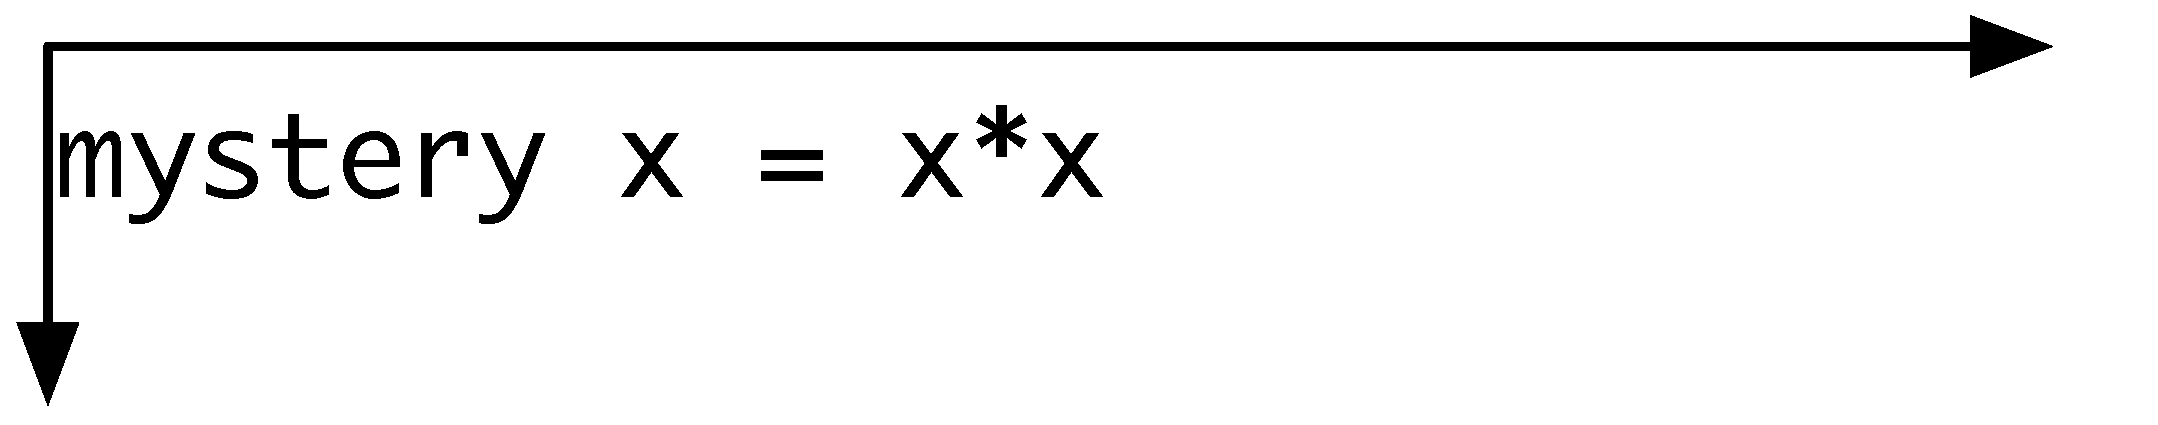
\includegraphics[width=2.3in]{Pictures/mystery1.pdf}
\end{center}
Whatever is typed in the box forms part of the definition \ldots
\begin{center}
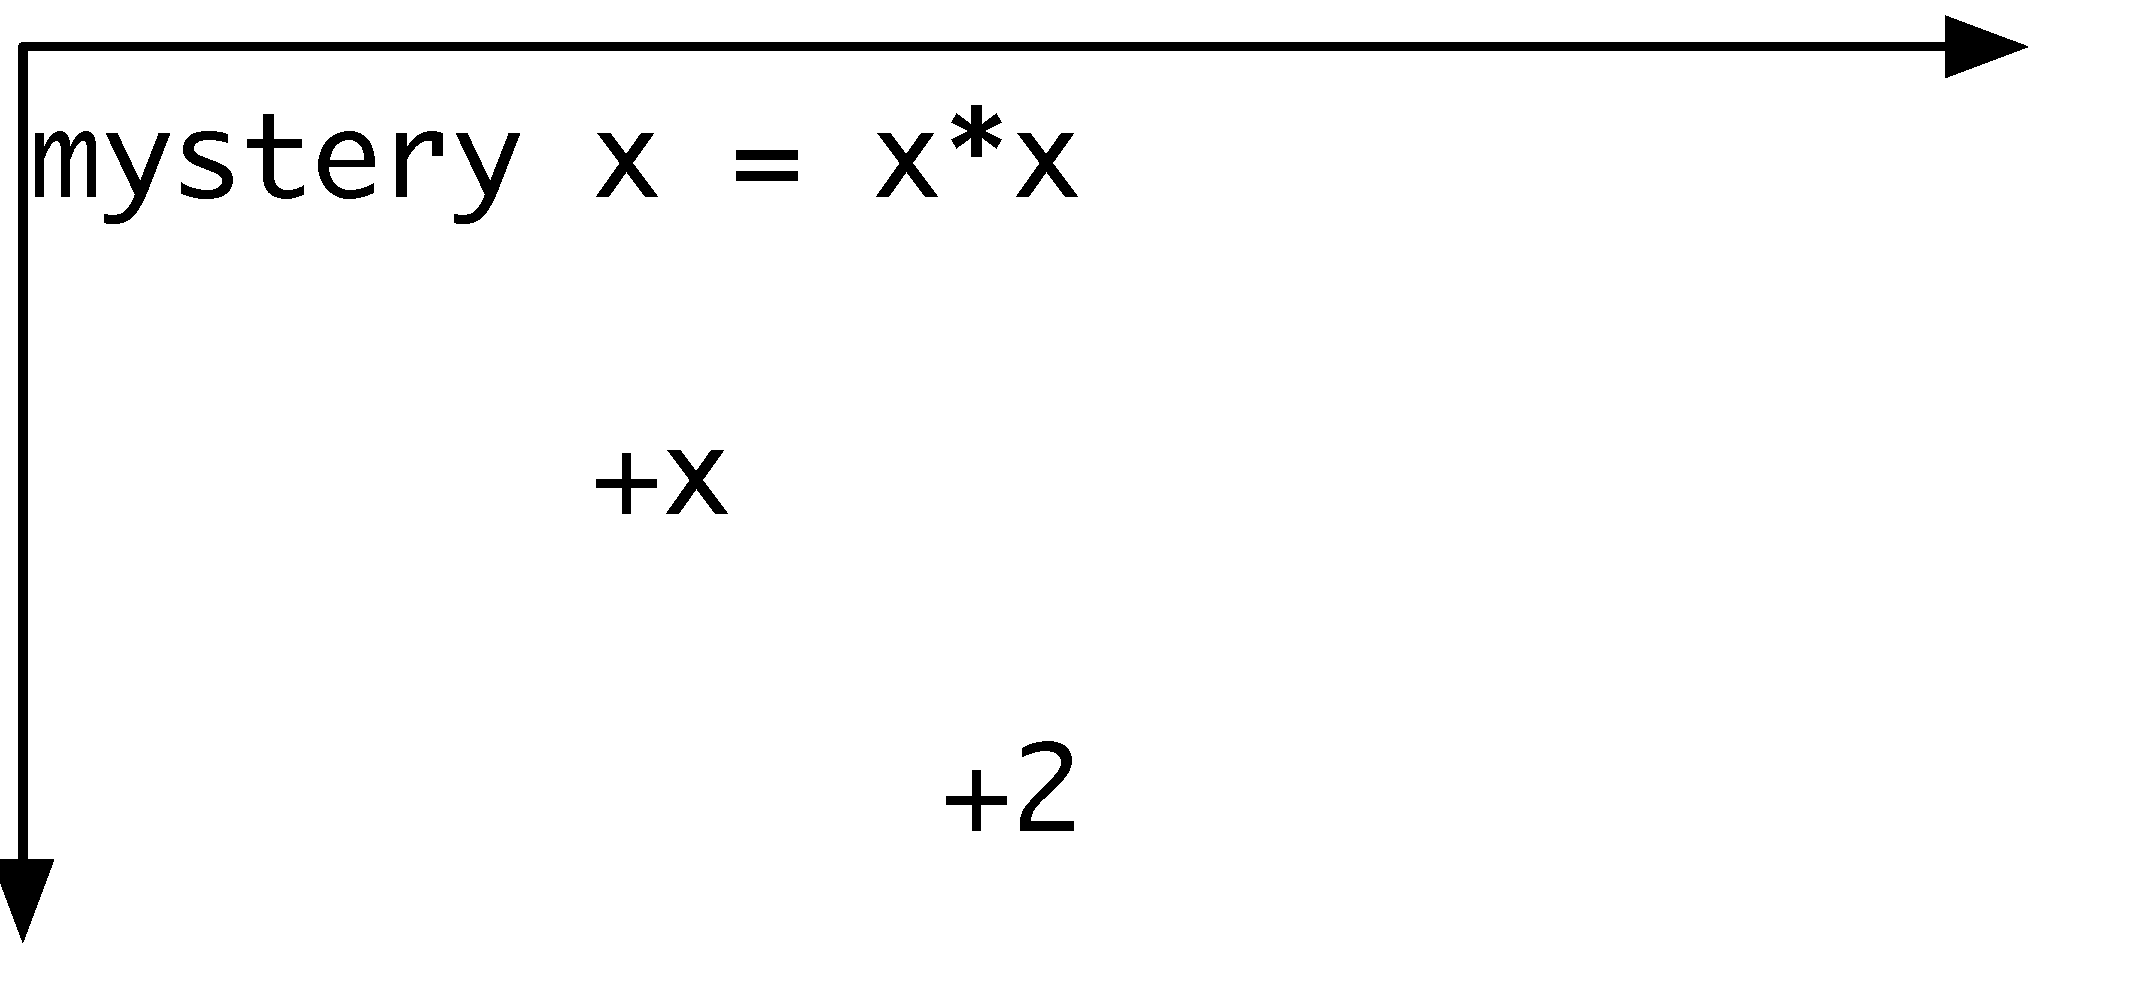
\includegraphics[width=2.3in]{Pictures/mystery2.pdf}
\end{center}
\ldots until something is found which is on the line
or to the left of the line. This
closes the box, like this
\begin{center}
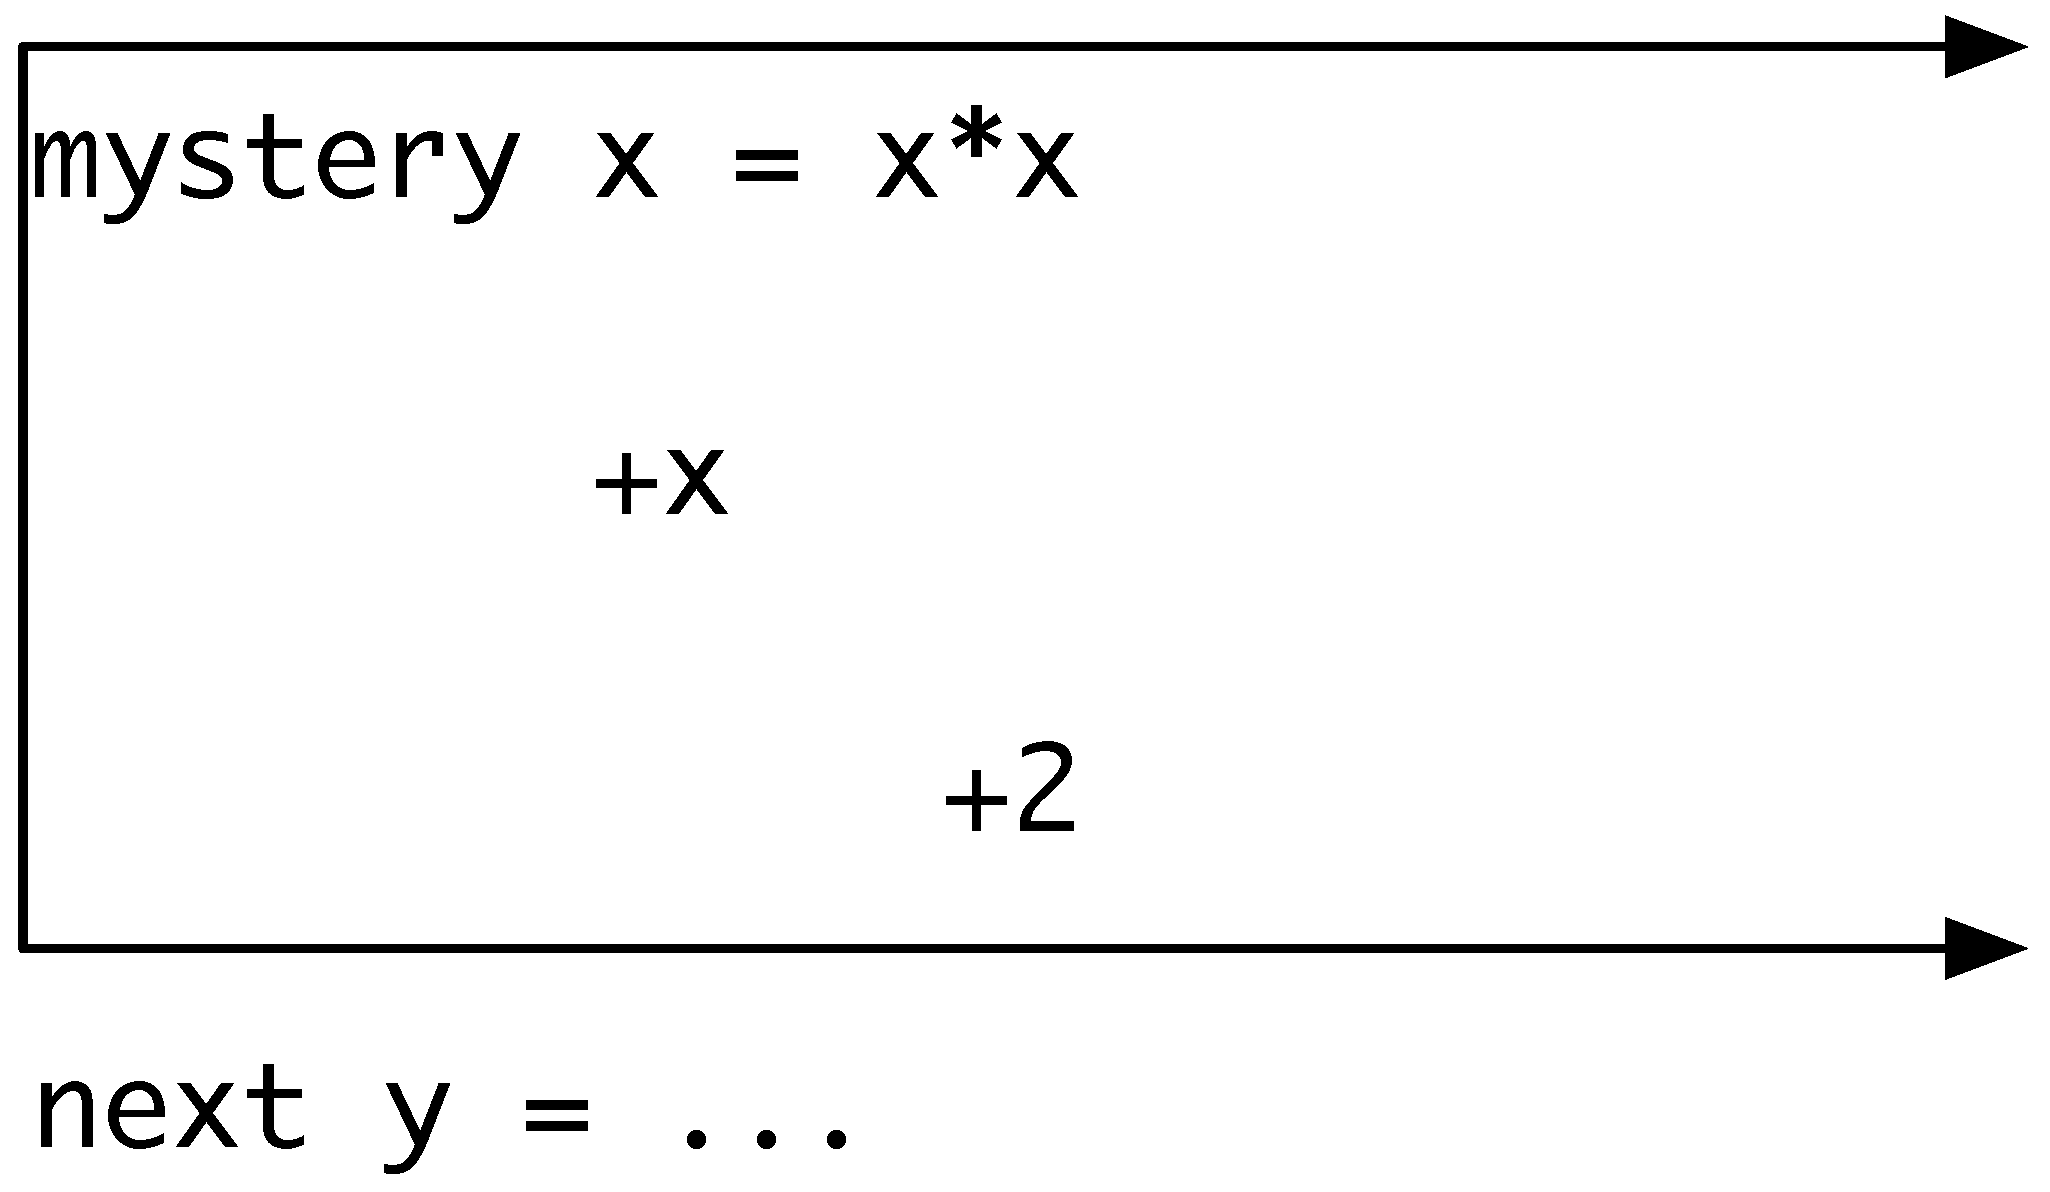
\includegraphics[width=2.3in]{Pictures/mystery3.pdf}
\end{center}
In writing a sequence of definitions, it is therefore sensible to give them
all the same level of indentation. In our scripts we shall always write
top-level definitions starting at the left-hand side of the page, and in
literate scripts we will indent the start of each definition by a single `tab'.

This rule for layout is called the \textbf{offside rule}\index{offside rule}
because it is
reminiscent of the idea of being `offside' in soccer.
The rule also works for conditional equations such as \texttt{max} and
\texttt{maxThree}
which consist of more than one clause.

There is, in fact, a mechanism in Haskell for giving an explicit end to part
of a definition, just as `\texttt{.}' does in English: the Haskell `end' symbol
is `\texttt{;}'. We can, for instance, use `\texttt{;}' if we wish to write more
\minx{;}
than one definition on a single line, thus:
\begin{alltt}
answer = 42 ;   facSix = 720 
\end{alltt}

\begin{figure}\index{errors!layout}
\beware{Layout errors}{\index{pitfalls!\texttt{;} in error message}%
If we break the offside rule like this:
\begin{alltt}
funny x = x+\\
1
\end{alltt}
we receive an error message like this:
\begin{alltt}
Chapter3.hs:33:0:

\ \ \ \ parse error (possibly incorrect indentation)
    
Failed, modules loaded: none.
\end{alltt}
which indicates that the indentation may well be the problem. The position 33:0 is the position of the digit \texttt{1}, which is in \emph{row} 33 and \emph{column} 0 of the file \texttt{Chapter3.hs}.
\index{errors!offside rule}
}\end{figure}

\subsection*{Recommended layout}
\index{layout!recommended}

The offside rule permits various different styles of layout. In this book 
for definitions of any size we use the form 
\begin{alltt}
fun \vone \vtwo \ldots \vn
  | \gone          = \eone     
  | \gtwo          = \etwo   
  \ldots
  | otherwise   = \er       ({\rm or}    | \gr      = \er)
\end{alltt}
for a \textbf{conditional equation}\index{conditional equation} built up
from a number of clauses.
In this layout, each \textbf{clause} starts on a new line, and the guards and results
\index{clause}
are lined up. Note also that by convention in this text we always specify the type
of the function being defined.
\index{conventions!types specified}

If any of
the expressions \texttt{\ei} or guards \texttt{\gi} is particularly long, then the
\index{guard}
guard can appear on a line (or lines) of its own, like this
\begin{alltt}
fun \vone \vtwo \ldots \vn
  | a long guard which may
    go over a number of lines 
       = very long expression which goes 
         over a number of lines
  | \gtwo       = \etwo         
  \ldots
\end{alltt}
If you use an editor which is Haskell-aware, e.g. emacs with Haskell mode, then the editor will help you to indent your code. In this particular case, hitting the tab key repeatedly will cycle through a set of suggested indentations of the line that you are currently working on, based on its contents.


\subsection*{Names in Haskell}

Thus far in the book we have seen a variety of uses of names in definitions
and expressions. In a definition like
\begin{alltt}
addTwo :: Int -> Int -> Int
addTwo first second = first+second
\end{alltt}
the names or \textbf{identifiers} \index{name}\index{identifier}
\texttt{Int}, \texttt{addTwo}, \texttt{first} and \texttt{second} are used to
name a type, a function and two variables. Identifiers in Haskell must begin
with a letter -- small or capital -- which is followed by an optional
sequence of letters, digits, underscores `\verb+_+' and single quotes.

The names used in definitions of values must
begin with a small letter, as must variables
and type
variables, which are introduced later. On the other hand, 
capital letters are used to begin
type names, such as \texttt{Int}; \textbf{constructors}\index{constructor}, such as
\texttt{True} and \texttt{False}; module names and also the names of  
type classes, which we shall encounter
below.

An attempt to give a function a name
which begins with a capital letter, such as
\begin{alltt}
Funny x = x+1
\end{alltt}
gives the error message:
\begin{alltt}
Chapter3.hs:32:0:
\ \ \ \ Not in scope: data constructor `Funny'
\end{alltt}
There are some restrictions on how identifiers can be chosen. There is
a small collection of \textbf{reserved words} which cannot be used; these
are\index{reserved words}
\begin{alltt}
case class data default deriving do else if import in infix
infixl infixr instance let module newtype of then type where
\end{alltt}
The special identifiers \texttt{as}, \texttt{qualified}, and
\texttt{hiding}\minx{as}\minx{qualified}\minx{hiding} 
have special meanings in certain contexts but can be
used as ordinary identifiers.

By convention, when we give names built up from more than one word, we
capitalize the first letters of the second and subsequent words, as in 
`\texttt{maxThree}'.
\index{conventions!capitalizing internal words}

The same identifier can be used to name both
a function and a variable, or both a type
and a type constructor; we recommend strongly that this is {\em not\/} done,
as it can only lead to confusion. 

If we want to \textbf{redefine} a name that is
already defined in the prelude or one of the libraries we have to \textbf{hide} that name on
import; details of how to do this are given on page \pageref{redefName}.

Haskell is built on top of the Unicode\index{characters!Unicode} character
description standard, which allows symbols from fonts other than those
in the ASCII standard.
These symbols can be used in identifiers and the like, and
Unicode characters -- which are described by a 16-bit sequence -- can be input 
to Haskell in the form \texttt{\bs{u}}\textit{hhhh} where each of the \textit{h} is a
hexadecimal (4 bit) digit. In this text we use the ASCII subset of
Unicode exclusively. 

\subsection*{Operators}
\label{operators}
\index{operator|(}

The Haskell language contains various operators, like \texttt{+}, \texttt{++} and
so on. Operators are \textbf{infix} functions, so that they are written between their
\index{operator!infix}
arguments, rather than before them, as is the case for ordinary functions. 

In principle it is possible to write all applications of an
operator with enclosing parentheses, thus
\begin{alltt}
(((4+8)*3)+2)
\end{alltt}
but expressions rapidly become difficult to read. Instead two extra
properties of operators allow us to write expressions uncluttered by
parentheses.

\subsubsection*{Associativity}
\index{operator!associativity of}
\index{associativity}

If we wish to add the three numbers \texttt{4}, \texttt{8} and \texttt{99} we can write
either \texttt{4+(8+99)} or \texttt{(4+8)+99}. The result is the same whichever we
write, a property we call the \textbf{associativity} of addition. Because of
this, we can write 
\begin{alltt}
4+8+99
\end{alltt}
for the sum, unambiguously. Not every operator is associative, however; what
happens when we write
\begin{alltt}
4-2-1
\end{alltt}
for instance? 
The two different ways of inserting parentheses give
\begin{alltt}
(4-2)-1 = 2-1 = 1\hfill{\rm left associative}
4-(2-1) = 4-1 = 3 \hfill{\rm right associative}
\end{alltt}
\index{associativity!left/right}
In Haskell 
each non-associative operator is classified as either left or right
associative. If left associative, any double occurrences of the operator
will be parenthesized to the left; if right associative, to the right. The
choice is arbitrary, but follows custom as much as possible, and in
particular `\texttt{-}' is taken to be left associative.

\subsubsection*{Binding powers}
\index{operator!binding power of}
 
The way in which an operator associates allows us to resolve expressions like
\begin{alltt}
2\^{}3\^{}2
\end{alltt}
where the same operator occurs twice, but what is done when two different
operators occur, as in the following expressions?
\begin{alltt}
2+3*4
3\^{}4*2
\end{alltt}
For this purpose the \textbf{binding power} or \textbf{fixity}
of the operators\index{fixity}\index{binding power}
need to be compared. \texttt{*} has binding power 7 while \texttt{+} has 6, so
that in \texttt{2+3*4} the \texttt{3} sticks to the \texttt{4} rather than the {\mi
2}, giving

\begin{alltt}
2+3*4 = 2+(3*4)
\end{alltt}
In a similar way, \texttt{\^{}} with binding power 8
binds more tightly than \texttt{*}, so

\begin{alltt}
3\^{}4*2 = (3\^{}4)*2
\end{alltt}
A full table of the associativities and binding powers of the predefined
Haskell operators is given in Appendix \ref{hsOps}. 
In the section `Do-it-yourself operators' below we discuss how
operators are defined in scripts and also how their associativity and binding
power can be set or changed by declarations. 

\begin{figure}[t]
\beware{Function application}{\index{function application}%
\index{pitfalls!function application}
Binding most tightly is function application, which is given by writing the
name of the function in front of its argument(s) thus:
\texttt{f \vone\ \vtwo\ \ldots\ \vn}. This binds more tightly than any other
operator, so that \texttt{f n+1} is interpreted as \texttt{f n} plus 
\texttt{1}, \texttt{(f n)+1}, rather than \texttt{f} applied to \texttt{n+1}, \texttt{f (n+1)}. 
If in doubt, it is sensible to
parenthesize each argument to a function application.

\medskip
Similarly, as `\texttt{-}' is both an infix and a prefix operator, there is
scope for confusion. \texttt{f -x} will be interpreted as \texttt{x} subtracted
from 
\texttt{f}, rather than \texttt{f} applied to \texttt{-x}; the solution again is to
bracket the argument, giving \texttt{f (-x)}.
}\end{figure}

\subsubsection*{Operators and functions}

Infix operators can be  written {\em before\/}
their arguments, by enclosing the operator in parentheses. We therefore have,
for example,
\begin{alltt}
(+) :: Integer -> Integer -> Integer
\end{alltt}
so that
\begin{alltt}
(+) 2 3 = 2 + 3
\end{alltt}
This conversion is needed later when we make functions into
arguments of other functions.
We can also convert functions into operators by enclosing the function name in
backquotes, thus \texttt{`name`}. We therefore have, using the maximum function
defined earlier,

\begin{alltt}
2 `max` 3 = max 2 3
\end{alltt}
This notation can make expressions involving \textbf{binary}\index{function!binary} or two-argument functions substantially easier to read.

The fixity and associativity of these operators can be controlled; see
Appendix \ref{hsOps}.

\subsubsection*{Do-it-yourself operators}
\index{operator!definitions of}

The Haskell language allows us to define infix operators directly in exactly the same way
as functions.
Operator names are built from the operator symbols which include the
ASCII symbols

\begin{alltt}
! \# \$ \% \& * + . / < = > ? \@ \bs{} \^{} | : - \twid
\end{alltt}
together with the Unicode symbols. An operator name may not begin with a
colon.

To define the operator \texttt{\&\&\&} as an integer minimum function, we
write

\begin{alltt}
(\&\&\&) :: Integer -> Integer -> Integer\minx{\&\&\&}
x \&\&\& y 
  | x > y       = y
  | otherwise   = x
\end{alltt}
The associativity and binding power of the operator can be specified; for details
see Appendix \ref{hsOps}.
\index{operator|)}
\index{syntax|)}

\begin{exercises}

\item Rewrite your solutions to the earlier exercises to use the recommended
layout.

\item Given the definitions
\begin{alltt}
funny x = x+x
 peculiar y = y
\end{alltt}
explain what happens when you remove the space in front of the {\mi
peculiar}.
\end{exercises}

\begin{summary}
This chapter has introduced the base types \texttt{Integer}, \texttt{Int}, \texttt{Float},
\texttt{Char} and \texttt{Bool} together with various built-in functions over them.
We have seen how Boolean expressions -- called guards -- allow
definitions which have various cases, and this was exemplified by the function
returning the maximum of two integer arguments. This definition contains two
cases, one which applies when the first argument is the larger and the other when the second is the larger.

Finally, we have seen how the layout of a Haskell program is
significant -- the end of a definition is implicitly given by the first
piece of program text `offside' of the start of the definition;  we
have also given an overview of operators in Haskell.

This material, together with what we have seen in earlier chapters,
gives us a toolkit which we can use to solve programming problems. In
the next chapter we will explore various ways of using that toolkit to
solve practical problems.
\end{summary}
%\end{document} 


